\chapter{The Arabic Script}
\label{ch:arabic}
\thispagestyle{empty}
\newpage
\refsection

The Arabic writing system is one of the geographically and chronologically most
widely used writing system in human history. It is the primary script for the
Arabic language, Farsi, Urdu, and multiple others on the Indian subcontinent.
Historically, it has been used to produce text in several additional languages,
ranging from Spanish to Chinese.

While its exact origins are still a topic of debate among researchers, it is
generally accepted that it evolved from either the Nabatean or the Syriac
script in the Middle East over the course of several centuries. Its maturation
is said to have occurred during the seventh century CE. Its diffusion is
closely linked to the spread of Islam, and several alphabetic variants as well
as calligraphic regional styles developed over time. Far from being a purely
liturgical script however, with a wealth of administrative records,
philosophical and scientific treatises, poetry, etc. existing.

From the perspective of DIA research, it would therefore be a misnomer to speak
of a single Arabic script. Persian epics in \emph{nastaʼlīq} style on highly
decorated marbled paper have little in common with \emph{naskh} private
correspondence or the angular rectilinear writing of early kufic Qur’anic 
codices. Each style, in combination with regional preferences as well as the
particular context of its utilization, presents specific challenges.

\section{The Principles of the Arabic Writing System}

The Arabic script is an \emph{abjad}, i.e. a consonantal writing system.
Similar to scripts for other semitic languages, only consonants and long vowels
are written. The reader has to infer short vowels from the context. Short
vowels and other marks for features such as doubling (gemination) and nunation
(adding a final n), can optionally be added (\emph{tashkīl}).
However, this is only systematic for transcriptions of the \emph{qurʼān}, and in
elementary texts for language learners. Like Syriac and Hebrew, the script is
written from right to left with the exception of numbers, which are written
from left to right.

\begin{table}[!htbp]
\begin{minipage}{\textwidth}
\begin{center}
\caption{The 28 letters of the Arabic abjad}
\label{tab:abjad}
\renewcommand*{\thefootnote}{\alph{footnote}}
\begin{tabularx}{\textwidth}{XXXXXp{2.6cm}} \toprule
\textbf{isolated} & \textbf{initial} & \textbf{medial} & \textbf{final} & \textbf{name} & \textbf{transliteration}\\
\midrule
\textarabic{ا} & \textarabic{ا} & \textarabic{ـا} & \textarabic{ـا} & ʾalif & ā\\
\textarabic{ب} & \textarabic{بـ} & \textarabic{ـبـ} & \textarabic{ـب} & bāʾ & b\\
\textarabic{ت} & \textarabic{تـ} & \textarabic{ـتـ} & \textarabic{ـت} & tāʾ & t\\
\textarabic{ث} & \textarabic{ثـ} & \textarabic{ـثـ} & \textarabic{ـث} & thāʾ & th\\
\textarabic{ج} & \textarabic{جـ} & \textarabic{ـجـ} & \textarabic{ـج} & jīm & j\\
\textarabic{ح} & \textarabic{حـ} & \textarabic{ـحـ} & \textarabic{ـح} & ḥāʾ & ḥ\\
\textarabic{خ} & \textarabic{خـ} & \textarabic{ـخـ} & \textarabic{ـخ} & khāʾ & kh\\
\textarabic{د} & \textarabic{د} & \textarabic{ـد} & \textarabic{ـد} & dāl & d\\
\textarabic{ذ} & \textarabic{ذ} & \textarabic{ـذ} & \textarabic{ـذ} & dhāl & dh\\
\textarabic{ر} & \textarabic{ر} & \textarabic{ـر} & \textarabic{ـر} & rāʾ & r\\
\textarabic{ز} & \textarabic{ز} & \textarabic{ـز} & \textarabic{ـز} & zayn & z\\
\textarabic{س} & \textarabic{سـ} & \textarabic{ـسـ} & \textarabic{ـس} & sīn & s\\
\textarabic{ش} & \textarabic{شـ} & \textarabic{ـشـ} & \textarabic{ـش} & shīn & sh\\
\textarabic{ص} & \textarabic{صـ} & \textarabic{ـصـ} & \textarabic{ـص} & ṣād & ṣ\\
\textarabic{ض} & \textarabic{ضـ} & \textarabic{ـضـ} & \textarabic{ـض} & ḍād & ḍ\\
\textarabic{ط} & \textarabic{طـ} & \textarabic{ـطـ} & \textarabic{ـط} & ṭāʾ & ṭ\\
\textarabic{ظ} & \textarabic{ظـ} & \textarabic{ـظـ} & \textarabic{ـظ} & ẓāʾ & ẓ\\
\textarabic{ع} & \textarabic{عـ} & \textarabic{ـعـ} & \textarabic{ـع} & ʿayn & ʿ\\
\textarabic{غ} & \textarabic{غـ} & \textarabic{ـغـ} & \textarabic{ـغ} & ghayn & gh\\
\textarabic{ف} & \textarabic{فـ} & \textarabic{ـفـ} & \textarabic{ـف} & fāʾ & f\\
\textarabic{ق} & \textarabic{قـ} & \textarabic{ـقـ} & \textarabic{ـق} & qāf & q\\
\textarabic{ك} & \textarabic{كـ} & \textarabic{ـكـ} & \textarabic{ـك} & kāf & k\\
\textarabic{ل} & \textarabic{لـ} & \textarabic{ـلـ} & \textarabic{ـل} & lām & l\\
\textarabic{م} & \textarabic{مـ} & \textarabic{ـمـ} & \textarabic{ـم} & mīm & m\\
\textarabic{ن} & \textarabic{نـ} & \textarabic{ـنـ} & \textarabic{ـن} & nūn & n\\
\textarabic{ه} & \textarabic{هـ} & \textarabic{ـهـ} & \textarabic{ـه} & hāʾ & h\\
\textarabic{و} & \textarabic{و} & \textarabic{ـو} & \textarabic{ـو} & wāwʾ & w/ū\\
\textarabic{ي} & \textarabic{يـ} & \textarabic{ـيـ} & \textarabic{ـي} & yāʾ & y/ī\\
%\multicolumn{5}{c}{\textbf{vowel and diacritical marks}}\\
%\midrule
%\textbf{letter} & & & & \textbf{name} & \textbf{transliteration}\\
%\textarabic{َ} & & & & fatḥah & a\\
%\textarabic{ُُ} & & & & ḍammah & u\\
%\textarabic{ِ} & & & & kasrah & i\\
%\textarabic{ْ} & & & & sukūn & zero-vowel\\
%\textarabic{ّ} & & & & shaddah & doubled consonant\\
%\textarabic{ًٌ/ً/ٍ}& & & & tanwīn & nunation marks\\
%\textarabic{ء}  &  & & & hamzah\footnote{\emph{Hamzah} is not considered as one of the canonical 28 letters but can nevertheless occur isolated and notsolely as an diacritic.}  & ʾ\\
\bottomrule
\end{tabularx}
\end{center}
\renewcommand\footnoterule{}
\end{minipage}
\end{table}

The original abjad used for writing Classical Arabic with its twenty-eight
distinctive phonemes contains only eighteen graphemes \emph{rasm}, causing the
same grapheme to represent up to five different phonemes. bāʾ, tāʾ, thāʾ, nūn,
and yāʾ share the same shape and are, depending on their position in the word,
written the same way. These glyphs are distinguished by dots placed above or
below them: one below for bāʾ, two above for tāʾ, three above for thāʾ, one
above for nūn, and two below for yāʾ. Correspondingly, dots are used to
differentiate ghayn and ʼayn, ṣād and ḍād, and jīm, ḥāʾ, and khāʾ. In contrast
to vocalization dotting is mandatory and is present in all but the earliest
Arabic texts. See table~\ref{tab:abjad} for an overview of the twenty-eight
letters of the standard Arabic abjad.

The Arabic script distinguishes itself from other widely used scripts such as
Latin, Cyrillic or Greek in that it does not have a printed form, i.e. a form
in which letters can be written separately. The cursive form is the only form
that exists, albeit it include a wide variety of styles. Similar to cursive
forms in other scripts, in Arabic individual letters will change shape
depending on their position within the word. Initial, medial, final and
independent shapes exist, to which one must add more complex placement rules
along the baseline, which depend on adjacent letters. Contrary to Latin, not
every letter in written Arabic can be connected to the letter that precedes or
follows it: roughly one fifth actually do not connect to the previous or following
letter. As a result, whitespace does not necessarily mark the beginning of a
new word, thus providing calligraphers with considerable freedom to vary
inter-word, inter-syllable, and inter-stroke spacing as desired. One could go
as far as abandoning word separation completely, in a kind of \emph{scripta
continua} \cite[pg. 15]{blair2006islamic}. However, even conventional
calligraphic practice displays spacing variation to some extent, which can
prove misleading for optical character recognition systems. 


Unlike many other scripts, Arabic does not know capital and lower case letter
forms and texts produced before the twentieth century CE do not contain
Western-style punctuation or layout such as commas, periods, question marks,
paragraphs, \dots. New sentences and questions are introduced using specific
words and phrases. Titles and headings are indicated as such by placing strokes
above them. After the ninth century CE, a variety of verse marks and signs
appear in Quranic manuscripts to help with recitation \cite{awad2015evolution}.

The script has been adapted for a fairly large number of other languages, most
prominently Persian and Turkish that do have some additional phonemes. Letter
forms are usually adapted by adding dots to graphemes representing similar
phonemes in Arabic, e.g. the Persian \emph{pe} is derived from \emph{bāʾ} by
writing two additional dots below. Sometimes graphemes were also modified more
directly such as the letter \emph{gāf} which is written by adding another bar
above the letter \emph{kāf}. Similar transformations exist for other languages
with some such as \emph{xiao'erjing}, the writing of sinitic languages in
Arabic script, changing it into a full alphabet by making the marking of short
vowels mandatory or creating additional letters for short vowels. The Unicode
standard alone lists more than a hundred additional graphemes for local
variants of the Arabic script.

\subsection{Text Justification}

As described Arabic does not share many features with other alphabetic scripts
but none of these are a fundamental obstacle to a modern OCR pipeline.  While
the cursive nature was seen as a major hindrance to older methods based on
character classifiers which require accurate segmentation to the character
level, newer segmentation-less methods are largely unaffected by this.
Nevertheless the variability in spacing, even on machine-printed text, is still
the primary source of errors (see section~\ref{s:whitespace}). Unfortunately,
the bundle of techniques employed to justify text, i.e. measures ensuring that
text ends flush with the left end of the writing space, require methods aware
of their function in all parts of the OCR pipeline.

Such techniques followed the proscription of hyphenation (i.e. splitting words
to facilitate line-wrapping) from the tenth century CE onwards. They were
created as a mean to avoid justification by whitespace alone, which often
produces visually unpleasant results (a phenomenon known as rivers in Western
typography). As a matter of fact, Western-style hyphenation is only visible in
certain early Koran manuscripts (albeit without explicit splitting markers such
as hyphens). It was most probably proscribed in Arabic script due to its
significant negative impact on legibility, especially if the second part of the
word is continued on a subsequent page.

One technique became prominent among later calligraphers working on hanging
styles such as the Persian \emph{nastaʼlīq}, in particular for poetry written
in hemi\-stiches. It consisted in stacking or heaping the last syllable or
penstroke above the left end of the line. It was particularly attractive for
Persian calligraphers to proceed this way, as many Persian words have similar
end letters. As such, the technique has but a negligible impact on legibility.
Similar stacking could be performed inside a line by changing the location and
size of diacritical marks \cite[pg. 14]{blair2006islamic}.

The existence of dislocated fragments into the margin represents another
challenge for OCR systems. Instead of heaping the last syllable on top of the
previous stroke, the fragment is placed in the margins, much like a marginal
note. These two practices add to the complexity of the layout analysis
component in the OCR pipeline. Firstly, the layout analysis system has to be
able to detect this type of fragments accurately. The methods presented in
part~\ref{part:la} have the potential to do so, at least with models specifically
trained to that purpose. Secondly, these types of fragments has to be
distinguished from bona fide marginalia and interlinear notes or translations
in order to be inserted in the textual output smoothly. This has to be done by
a reading order determination algorithm which knows of their existence. If the
algorithm is naïve and assumes that the text follow a top-to-bottom order, it
will insert this type of fragments before the text of the line it is associated
with, i.e. in reverse order. This is true even if other marginalia are correctly
filtered through previous classification using a segmenter. Unfortunately,
reading order determination is a notoriously under-researched task in DIA. ome
tentative approaches, such as \cite{dejean2019versatile} that could serve as a
basis for versatile reading order determination methods, exist, but all
practically available OCR system operate on simple heuristics.

Two other practices should have their existence mentioned here, although their
impact on OCR performance is likely to be limited. The first practice consists
in stretching the letter body or the connections between individual letters. It
is interchangeably known as either \emph{taṭwīl} or \emph{kashida}, although
certain typography-related publications use \emph{kashida} only to refer to the
stretching of the letter body. This practice is visible in most Arabic styles,
albeit its exact placement differs among scripts. Not only can it be used for
justification but also to highlight the beginning of a verse, a heading, etc. 

The second practice consists of the upward curving of the baseline, trading
horizontal with vertical space. However, conventional layout analysis methods
tend to model lines as either rectangular bounding boxes or
undirected\footnote{Undirected in the sense that there is no defined text
orientation or direction contained within the polygon. Only a bounding polygon
is given.} polygons. The presence of an upward curving in the baseline (and
more generally the presence of any slanted line) is likely to degrade the
results. This is due to the protruding of other lines into the bounding box, or
to height normalization, which results in insufficient text size as
demonstrated in figure~\ref{fig:intro_bbox}. Segmenters founded on the baseline
paradigm, like the ones presented in chapters~\ref{ch:hip} and \ref{ch:icfhr},
do not suffer from this problem as they allow the projection of arbitrarily
shaped lines onto a straight line.

\section{Supports and Production}

The question of supports is often neglected in the OCR research community.
While processing inscriptions in stone or clay tablets present unique and
obvious challenges, the difficulties that may arise from subtle differences of
supple writing surfaces are usually disregarded. Papyrus and parchment were
used as writing material until they were replaced by cheaper paper after the
8th century. Richly adorned specialty papers, which were often used in high
status documents, are of particular interest to Computer Vision experts.

We also include in the present dissertation a short discussion on inks, dyes
and techniques of illumination, not only because they cause a number of
difficulties to OCR systems, but also because of the potential for large scale
and automatized analysis across collections that DIA methods may offer in the
future. 

\subsection{Supports}

Paper, parchment and papyrus are the three main supports used in the Islamic
world, although paper largely overshadows parchment or papyrus in terms of
usage, whether it be geographically or chronologically.

Papyrus has been a support for writing since at least 3000 BCE. It is a
light-colored, smooth, and flexible material which is manufactured using
\emph{Cyperus papyrus}, a three-to-six meter high Egyptian water reed. The
production process goes as follow: first, the reed stalk is cut into halves,
and the pulp is extracted into thin strips. Strips are then arranged into
rectangular sheets made of two perpendicular layers, and left to dry under the
sun.  Once dried, sheets are smoothed with a mallet, prior to their polishing
by means of a shell or an ivory. Sheet sizes could vary considerably, although
it wasn’t uncommon for their width to be around 20-30 cm, and their length
around 30-40 cm.

Following polishing, individual sheets are glued end-to-end, while overlapping
joints are smoothed again. Sheets are then rolled with the horizontal fibers on
the inside. Like in the pre-Islamic period, a roll was composed of twenty
sheets, although papyrus would also be sold in smaller pieces (most commonly as
one-sixth of a roll). To protect rolls from wear, a thicker gauge strip of
papyrus called a \emph{protokollon} was attached to their top before use.

Scrolls were in use up until the early eighth century CE. However, the majority
of the documents that survived are either in codex form or are single sheet
documents\cite[pg.30]{deroche2006islamic}. While some literary papyri are
known, most Arabic papyri were documentary in nature, and contained letters,
edicts, and contracts. It is likely that papyrus was a rather expensive writing
material. They were rapidly phased out after the introduction of cheaper paper,
and production ceased in the eleventh century CE
\cite[pg.193-194]{gacek2009arabic}. 

Papyri raise two problems for DIA methods. They are brittle and fragile, which
frequently results in significant degradation (figure~\ref{fig:papyrus}).
Besides, with age, they darken to a point where their ink often becomes almost
illegible. The ageing process also increases contrast between fibers, which
further complicates any attempt at distinguishing the text from its background.
Hand-crafted binarization methods have been developed for the highly degraded
Dead Sea Scrolls \cite{dhali2017digital, lavee2013computer} but processing
remains difficult. Papyri length in scroll form poses another, perhaps more
minor, problem.  While many modern neural network-based methods can be adapted
to patchwise operation with minimal loss of accuracy, a number of them (in
particular layout analysis) perform better with global context. 

\begin{wrapfigure}{O}{0.7\textwidth}
        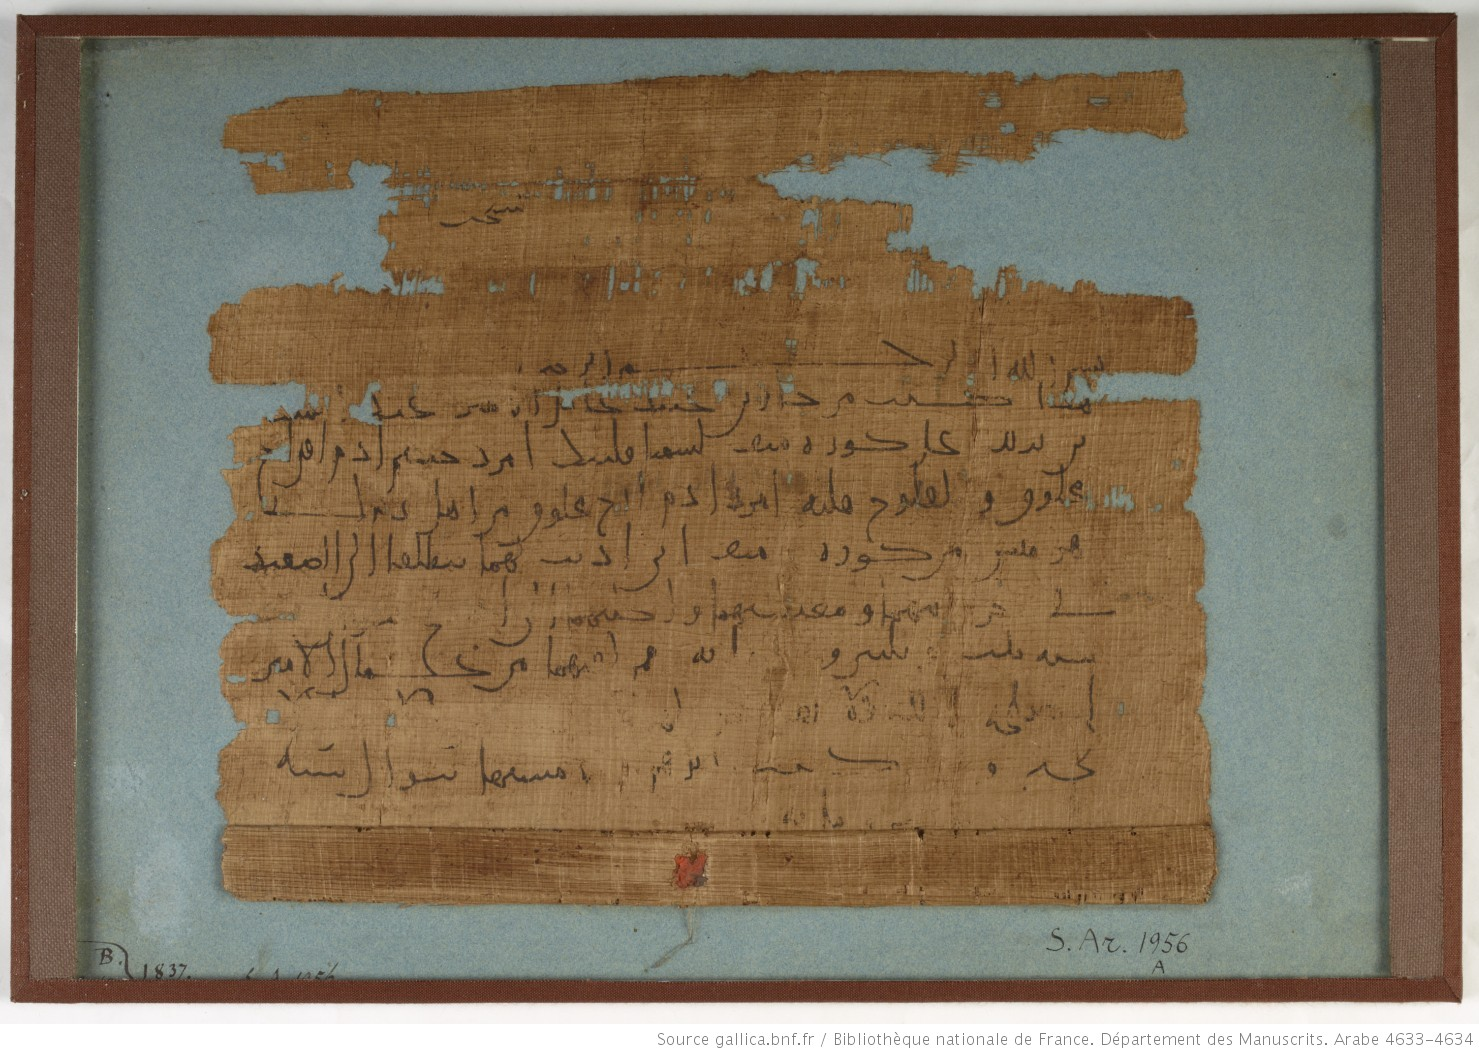
\includegraphics[width=0.68\textwidth]{images/4644.jpg}
	\caption{An Arabic papyrus showing both visible fibers and typical
	deterioration of the writing surface (BnF Arabe 4634).}
        \label{fig:papyrus}
\end{wrapfigure}

The second writing surface in wide\-spread use before the introduction of paper
in the Islamic world was parchment. Parchment is a carefully processed un- or
minimally tanned animal skin; fundamentally it can be procured from a variety
of animals and its production is not limited to a particular geographic area as
papyrus. Goat, calf, donkey, and gazelle skins, although these have never been
corroborated by testing, are mentioned as sources but the most common was sheep
skin~\cite[pg. 44]{blair2006islamic}. Its use in the East extends to time
memorial although no dated Arabic manuscripts from before the ninth century CE
have survived~\cite[pg.33]{deroche2006islamic}. 

Parchment is manufactured as follows. First, a basic solution (made from lime
or dates) is used to remove the hair from the hide.  Second, residual flesh and
fat is scraped from the flesh side of the hide using a blade. It is then placed
in a wooden frame to stretch it and dry it. Finally, an abrasive stone is used
to smoothen the surface and equalize the texture of both the flesh and hair
sides. Chalk is applied to control ink bleeding. Sometimes, parchments could be
dyed with blue indigo or yellow saffron. The most famous example of this
practice is the Blue \emph{Qurʼān} , dating back from the tenth century CE \cite[pg.
195-196]{gacek2009arabic}.

The ease with which previously used parchments could be reemployed by washing
or scraping off existing writing is an important consideration for both
humanists and computer vision researchers. Known as palimpsests, this practice
is attested both in the literature and by several surviving exemplars.
Considerable time could elapse between the moment the first layer was written
on and the moment it was covered with a second one. Examples of Arabic text
over a lower layer written in another script such as Greek or Syriac
exist~\cite[pg. 43-46]{deroche2006islamic}. While it was the complete removal of
the initial writing that was intended, oftentimes the lower layer remains
visible to a certain extent. 

The task of separating the writing to decipher both texts requires immense
skill, which can be aided by costly multispectral
imaging~\cite{easton2003multispectral}. However, it has not gathered much
research interest in the DIA community. \cite{starynska2017methods} (one of the
few publications on the topic) points out that existing methods need
substantial improvement. Parchment could also be recycled in other ways, e.g.
in bookbinding or as protective covers to loose quires, not quite unlike
papyrus \emph{protokollon}~\cite[pg. 46]{deroche2006islamic}.

Paper was invented in China in 105 CE by the Han courtier Cai Lun. Its
introduction to the Islamic world is attributed traditionally to a Muslim
military victory on the river Talas (modern-day Kazakhstan) in July 751 CE.
Allegedly, a number of Chinese papermakers were made war prisoners following
the battle and dispatched to Samarqand to set up paper mills. Details of this
story can certainly be disputed, however there are etymological hints that
knowledge of papermaking was received through Central Asia~\cite[pg.
45]{blair2006islamic}. Paper proved to be significantly cheaper than its
alternatives, and rapidly replaced papyrus and parchment as the writing surface
of choice. By 794 CE, paper mills were established in Baghdad. Its use by the
Abbasid Caliphate administration was mandated in 808 CE. By the ninth century,
paper was produced in Egypt. By the tenth century it had reached the Maghreb,
and by the twelfth century it was produced in Damascus and in Spain~\cite[pg.
51]{deroche2006islamic}.

Apart from economical reasons paper had other benefits: it absorbes ink so
writing could not easily be erased~\cite[pg. 45]{blair2006islamic}, it is less
brittle than papyrus with a more uniform coloration, and can be easily tinted
and decorated.

The availability of inexpensive writing material produced a flurry of literary
activity in the ninth century in a broad range of subjects, from theology to
the natural sciences. Books were soon copied on paper. Quranic manuscripts,
however, continued to be written on parchment until the late tenth century CE,
and exemplars could be found in the Maghreb and West Africa up until the
fourteenth century CE.

Descriptions of the papermaking process in the Islamic world are sparse and
lack clarity. The general process seems to have included suspension of
cellulose fibers for draining through a screen, followed by drying. This
resulted in a fiber mat is called paper. Sources of fibers could vary
considerably: they could either be liberated from virgin plant material through
a combination of heat, beating, and chemical means such as fermentation or
acids, or originate from waste material such as rags, old ropes, etc. Primary
material was then suspended in water to soak, prior to collection and draining
in a mold. An account from modern-day Tunisia describes an example of
papermaking from raw flax on a floating screen. On the other hand, analysis of
extant specimens shows that waste materials, such as rags from cotton and linen
or ropes, were primarily used. Before use, paper has to be sized with a mixture
of starches and egg white and burnished to prevent the ink from bleeding
excessively~\cite[pg. 44-45]{bloompaper}.

\begin{figure}[h!tp]
        \centering
	\begin{subfigure}[t]{0.3\textwidth}
		\centering
		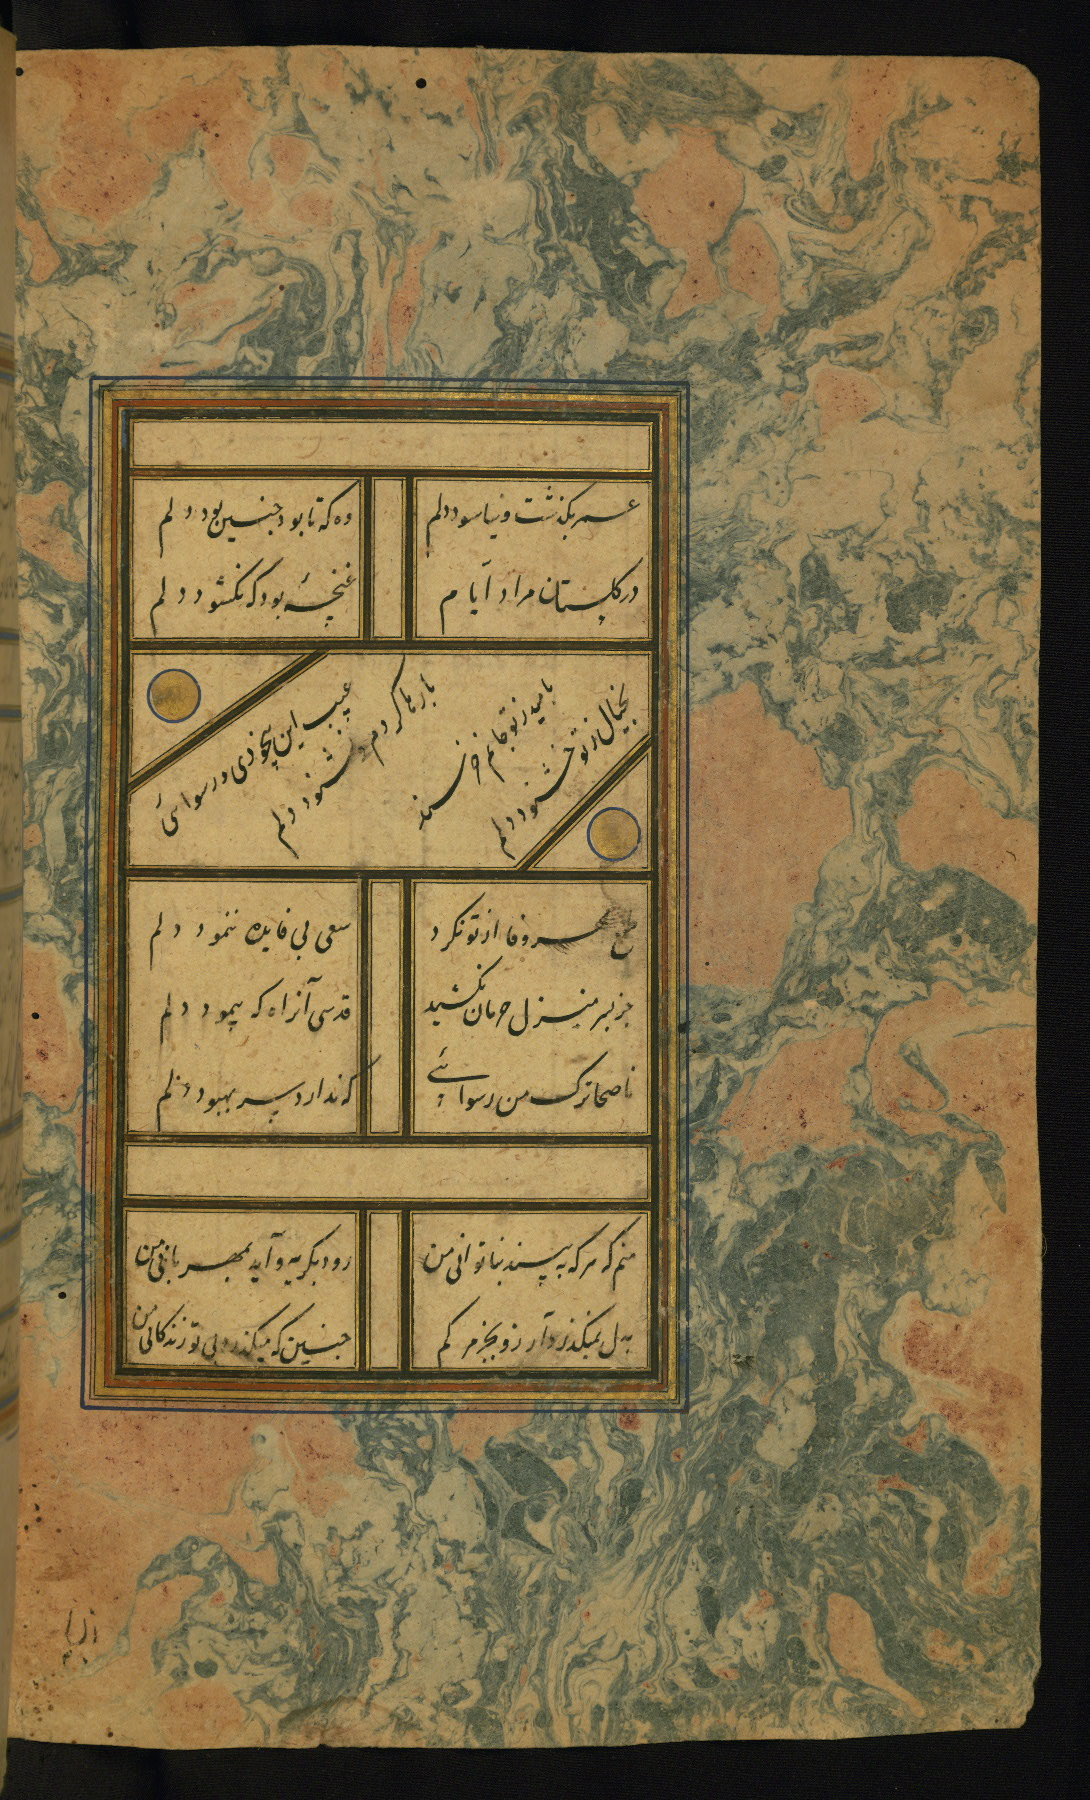
\includegraphics[height=0.3\textheight]{images/W654_000010_sap.jpg}
		\caption{Example of marbled paper (Walter W.654, fol. 1b)}
                \label{fig:ara_marble}
        \end{subfigure}
	\hfill
	\begin{subfigure}[t]{.33\textwidth}
		\centering
                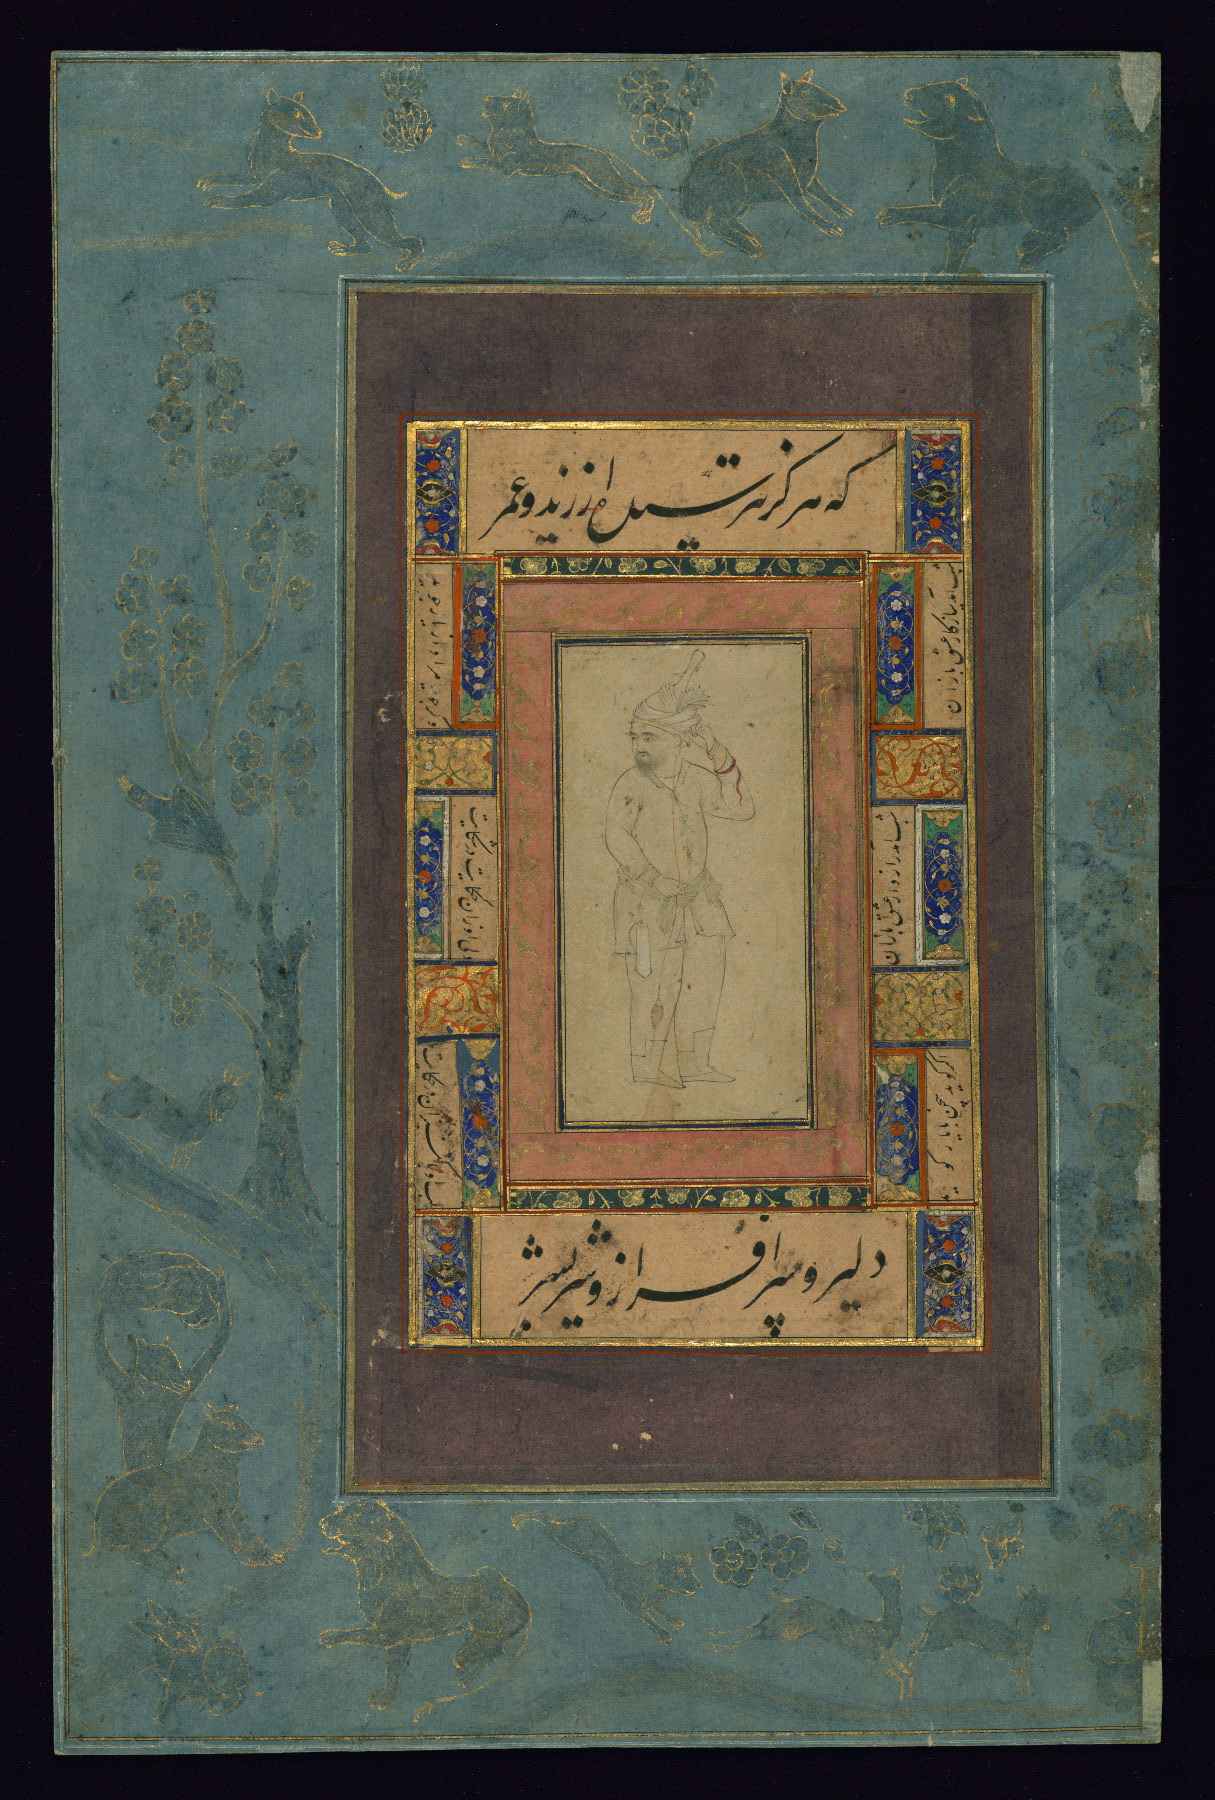
\includegraphics[height=0.3\textheight]{images/W746_000001_sap.jpg}
		\caption{A page with an outer border made of blue-tinted paper and an inner rose-tinted paper (Walters W.746).}
                \label{fig:ara_blue}
        \end{subfigure}
	\hfill
	\begin{subfigure}[t]{.3\columnwidth}
		\centering
                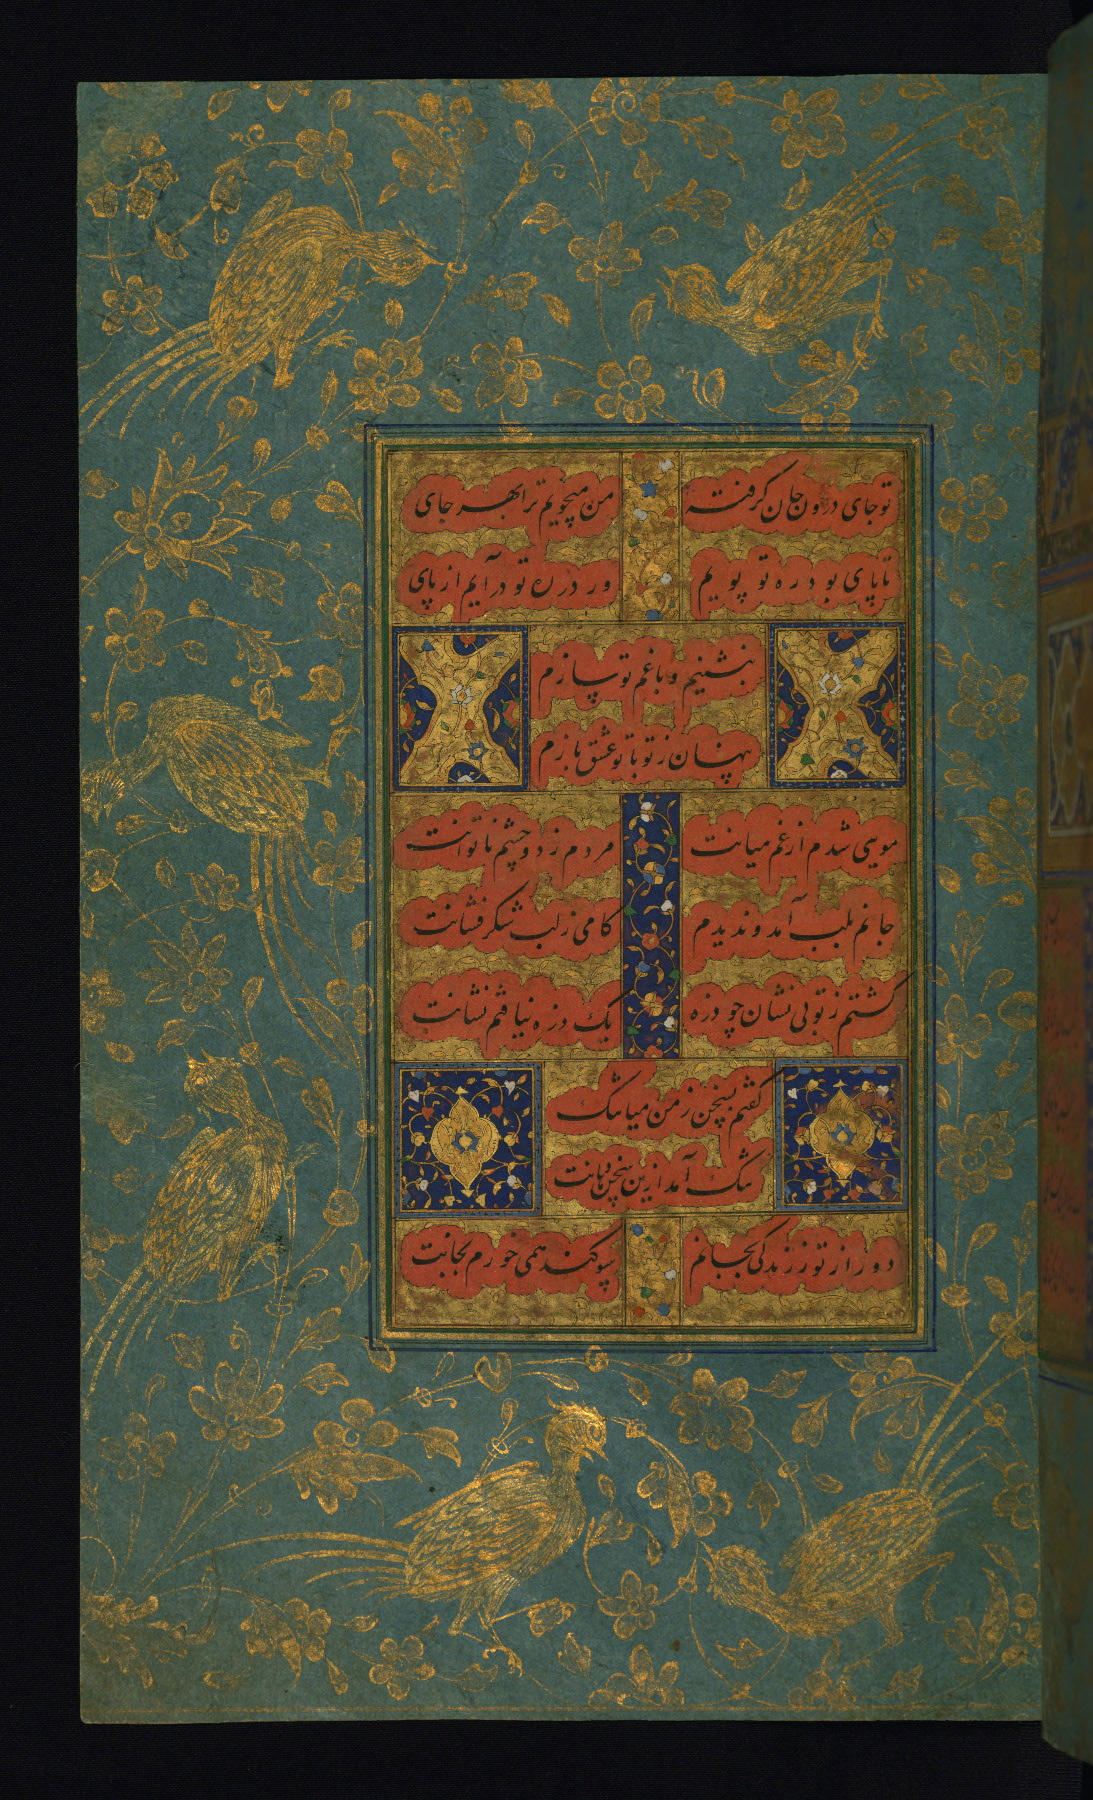
\includegraphics[height=0.3\textheight]{images/W651_000009_sap.jpg}
		\caption{Illumination in gold on blue-tinted border with text written on orange-tinted paper (Walters W.651, fol. 2a).}
                \label{fig:ara_orange}
        \end{subfigure}
        \caption{Decorated papers}
\end{figure}

A particularly impressive practice that often presents a challenge to modern
DIA methods are specially prepared papers used for many fine manuscripts.
Pre-modern papers retained the color of the source of the fibers, a fact that
was used in European manufacture to produce colored papers, most often various
hues of brown, but could also be tinted or dyed (figure~\ref{fig:ara_blue}).
The preference for tinted papers was probably initially fueled by colored
imports from China but Iranian artists started developing techniques to make
colored, gold-decorated, and marbled papers by the thirteenth century CE.
Popular colors were red or orange, and Persian treatises of the time list a
plethora of recipes to obtain these colors. Gold-sprinkled paper
(figure~\ref{fig:ara_orange}) was utilized throughout the Eastern Islamic lands
by the late fifteenth century CE with even more elaborate gold painting
incorporating arabesques coming into fashion from the sixteenth century onward
at the Safavid, Mughal, and Uzbek courts. Such gold-decorated papers were
mainly used in scrapbook albums of calligraphy and paintings to unify the
disparate contents into a single book. 

Two other techniques rose in popularity after the fifteenth century CE: marbled
papers (figure~\ref{fig:ara_marble}) and paper cuts. While the marbling
produced by slipping a sheet of paper over a bath of carefully swirled colorant
cause the same issues to DIA methods as other decorated margins, paper cuts are
likely more complicated.  Cut-out calligraphy, either collage, i.e. placing
cut-out letters on a contrasting background, or decoupage, i.e. mount a sheet
with cut out letters above a differently colored one, allows larger variation
in coloration than purely ink-based writing. Artists were often skilled in more
than one of these techniques and they are often employed together. Works such
as a collection of forty hadith for the Ottoman prince Mehmed in 1540 CE,
contain text in both \emph{taw'qī} and \emph{nastaʼlīq} script, pasted in gold,
white, or light blue on deep-rose or olive grounds. The margins on some pages
are kept plain, others gold-sprinkled, others again marbled~\cite[pg.
52-56]{blair2006islamic}. The sheer variety of text production and decoration
techniques a single manuscript can display is an important challenge to DIA
systems.

\subsection{Writing Instruments and Inks}

The Arabic script is traditionally written with a reed pen whose front had been
trimmed with a special pen knife to create a nib. Depending on the script’s
desired width, the nib can be slit one or several times at its end, depending
on the script’s desired width. Multiple nib cuts exist. Straight and oblique
cuts change the thickness of strokes at certain angles. Nonetheless, the
association of cut angles and scripts seems to have been largely a matter of
scribal preference\cite[pg. 42]{gacek2009arabic}.

Brushes were used primarily during the decoration process, for example to paint
in the margins or for gilding. In the fourteenth century CE, Chinese Muslims
developed the rounded, flowing \emph{ṣīnī} script to adapt Arabic writing to
Chinese calligraphy’s instruments and conventions. In certain cases, it went as
far as changing the directionality of writing to top-to-bottom \cite[pg.
29-0]{ghoname2012sini}.

More than pens and brushes, the type of ink and pigment used for writing is an
important element when performing document image analysis. Three kinds of black
or brown inks were commonly used: carbon-based inks, so-called mixed inks, and
iron gall inks. Compound inks were also common in the medieval period~\cite[pg.
62-63]{blair2006islamic}. All of them were known since Antiquity in the area
that would later be known as the Islamic world. Carbon inks are attested as far
back as the second millenium BCE in Egypt. The first recipes for mixed inks
date back to the third century BCE and iron gall inks were in use by the fifth
century CE~\cite{christiansen2017manufacture}.

Carbon inks are more commonly known as India inks. They are composed of fine
soot or finely ground charcoal mixed with some kind of binder, such as oil,
gums, or shellac. For portability purposes, they often took the form of a solid
stick, which was grounded and mixed with water before use. In the Muslim world,
the main source of carbon for inks was from the combustion of vegetable matter
such as rice, olives, chick-peas or various oils. The most common binders were
gum arabic and honey~\cite[pg. 133]{gacek2009arabic}. This type of ink
preparation adheres to the writing surface only superficially. It can easily be
washed off with water; it smudges easily if kept in humid conditions and can
peel off over time. So-called mixed inks represent an improvement. They can be
prepared by adding copper, lead or iron salts to carbon ink. The addition of
extra components, which acted as drying agents, was intended to increase ink
adherence to paper. On the other hand, iron gall inks do not contain any
carbon. When applied to paper, the ink undergoes an oxidation process, thus
forming an insoluble ferric tannate pigment. It is prepared by mixing tannic
acid (extracted from gallnuts), vitriol (ferric sulfate), and a binder such as
gum arabic. Unlike other types of ink, it penetrates the writing surface and is
indelible~\cite{christiansen2017manufacture}. Iron gall inks have a major
drawback, however. They are acidic in nature and tend to fade over time. As a
result, manuscripts written with iron gall ink are often damaged due to acid
burns, to the point of being illegible to human readers and computer vision
methods alike~\cite[pg. 145]{gacek2009arabic}

Colored inks were used by scribes and calligraphers as accent colors for
rubrics, vocalization, and other decoration. Red, green, and yellow were most
common. Pigments used for ink manufacturing have not been studied
systematically, but red inks usually contained cochineal, vermillion, and red
lead pigments; blue inks contained lapis lazuli and azurite; and verdigris can be
found in green inks. There is also substantial regional differences, as
pigmentation and coloration traditions differ widely from east to west
~\cite[pg. 63]{blair2006islamic}. This kind of coloration does not pose much of
a challenge to modern DIA methods, although pipe\-lines employing binarization
might encounter substantial degradation as the most commonplace binarization
algorithms perform quite poorly on mixed-color texts. Metallic inks are more
troublesome. This is not due to their inherent illegibility; but rather to the
low contrast that scanned documents showcase (see
figure~\ref{fig:ara_muhaqqaq}). For metallic inks, fine metals (e.g. gold,
silver, copper) were used in at least two different ways. The first way
consisted of liquid inks, which were made of metal flakes suspended in a
binder~\cite[pg. 225-227]{raggetti2019inks}. Secondly, powdered flakes could be
dispersed onto glue, to be subsequently burnished and ringed with other colors.
The latter technique produces writing that is prone to degradation, as
disintegration of the glue has caused flakes to fall off~\cite[pg.
63]{blair2006islamic}.

\section{Styles}

A large number of both formal and informal calligraphic styles have been
devised over the centuries. While informal styles naturally evade uniform
classification, formal styles can be divided into two groups: styles that are
recognized throughout the Muslim world (such as \emph{naskh}), and styles that
are limited to a certain geographical region or only used to write specific
languages, such as the North African and Iberian \emph{maghribī} or the Persian
\emph{nastaʼlīq}. 

Arabic styles can be defined by elements such as~\cite[pg.
242-243]{gacek2009arabic}:

\begin{description}
	\item[Line of writing] whether all words sit completely on the
			       baseline, descend onto it as in
			       \emph{nastaʼlīq}, curve upwards toward the end,
			       or are slanted.
	\item[Ascender and descenders] vertical, slanted or curved
	\item[Nib width] especially in relation to script size.
	\item[Shading] i.e. contrast between thin and thick strokes.
	\item[Vocalization] Some scripts require a different pen for vocalization.
	\item[Ligatures] The presence of unauthorized connections between letters.
	\item[Contractions] The presence of assimilated (omitted) letter forms.
	\item[Characteristic letterforms] such as straight, wavy, or slanted \emph{ʾalif}
\end{description}

The two earliest styles that emerged in the seventh century CE are
\emph{ḥijāzī} (figure~\ref{fig:ara_hijazi}) and kufic
(figure~\ref{fig:ara_kufic}. Both are somewhat confusingly named after early
Islamic intellectual centers (Hijaz and the city Kufa in southern Iraq) and a
variety of alternative terms such as Early Abbasid have been proposed. As
canonicalization was fairly low the terms do not refer singular hands but to
families of styles that were used mainly to transcribe copies of the
\emph{qurʼān}. One taxonomy divides them into six and four groups for the kufic
and \emph{ḥijāzī} family respectively. Either is notably more angular than
later round styles.  Hijazi being in use from 650 CE it was surplanted by kufic
by the beginning of the eighth century CE. While elaborate, highly decorated
manuscripts in the kufic style survive, the number of surviving Hijazi
fragments is very low and their appearance is utilitarian~\cite[pg. 98,
124]{gacek2009arabic}.

\begin{figure}[h!tp]
        \centering
        \begin{subfigure}{\textwidth}
		\centering
		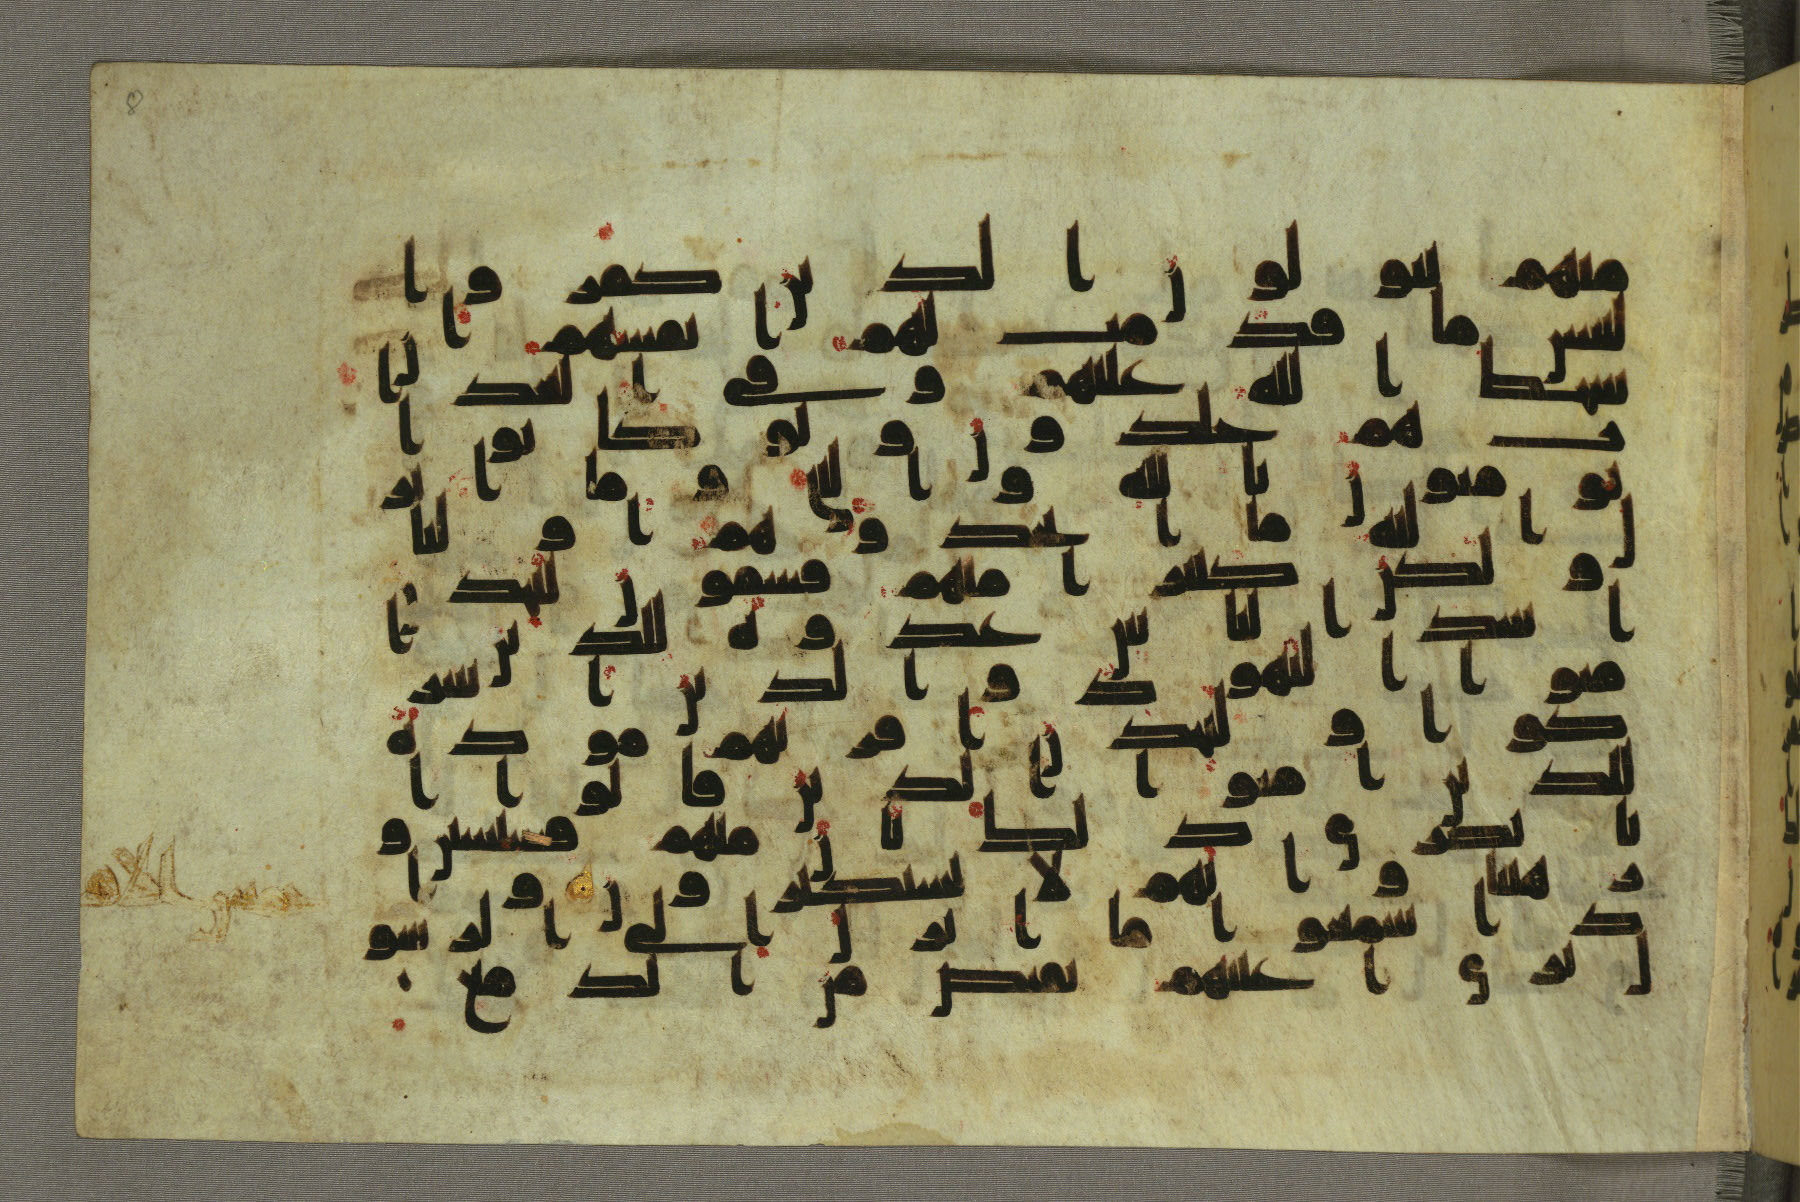
\includegraphics[width=\textwidth]{images/W552_000024_sap.jpg}
		\caption{Ninth century CE \emph{qurʼān} in Kufic or Early Abbasid script (Walters W.552, fol. 8a)}
                \label{fig:ara_kufic}
        \end{subfigure}
        \vskip\baselineskip
	\begin{subfigure}[t]{.4\textwidth}
		\centering
                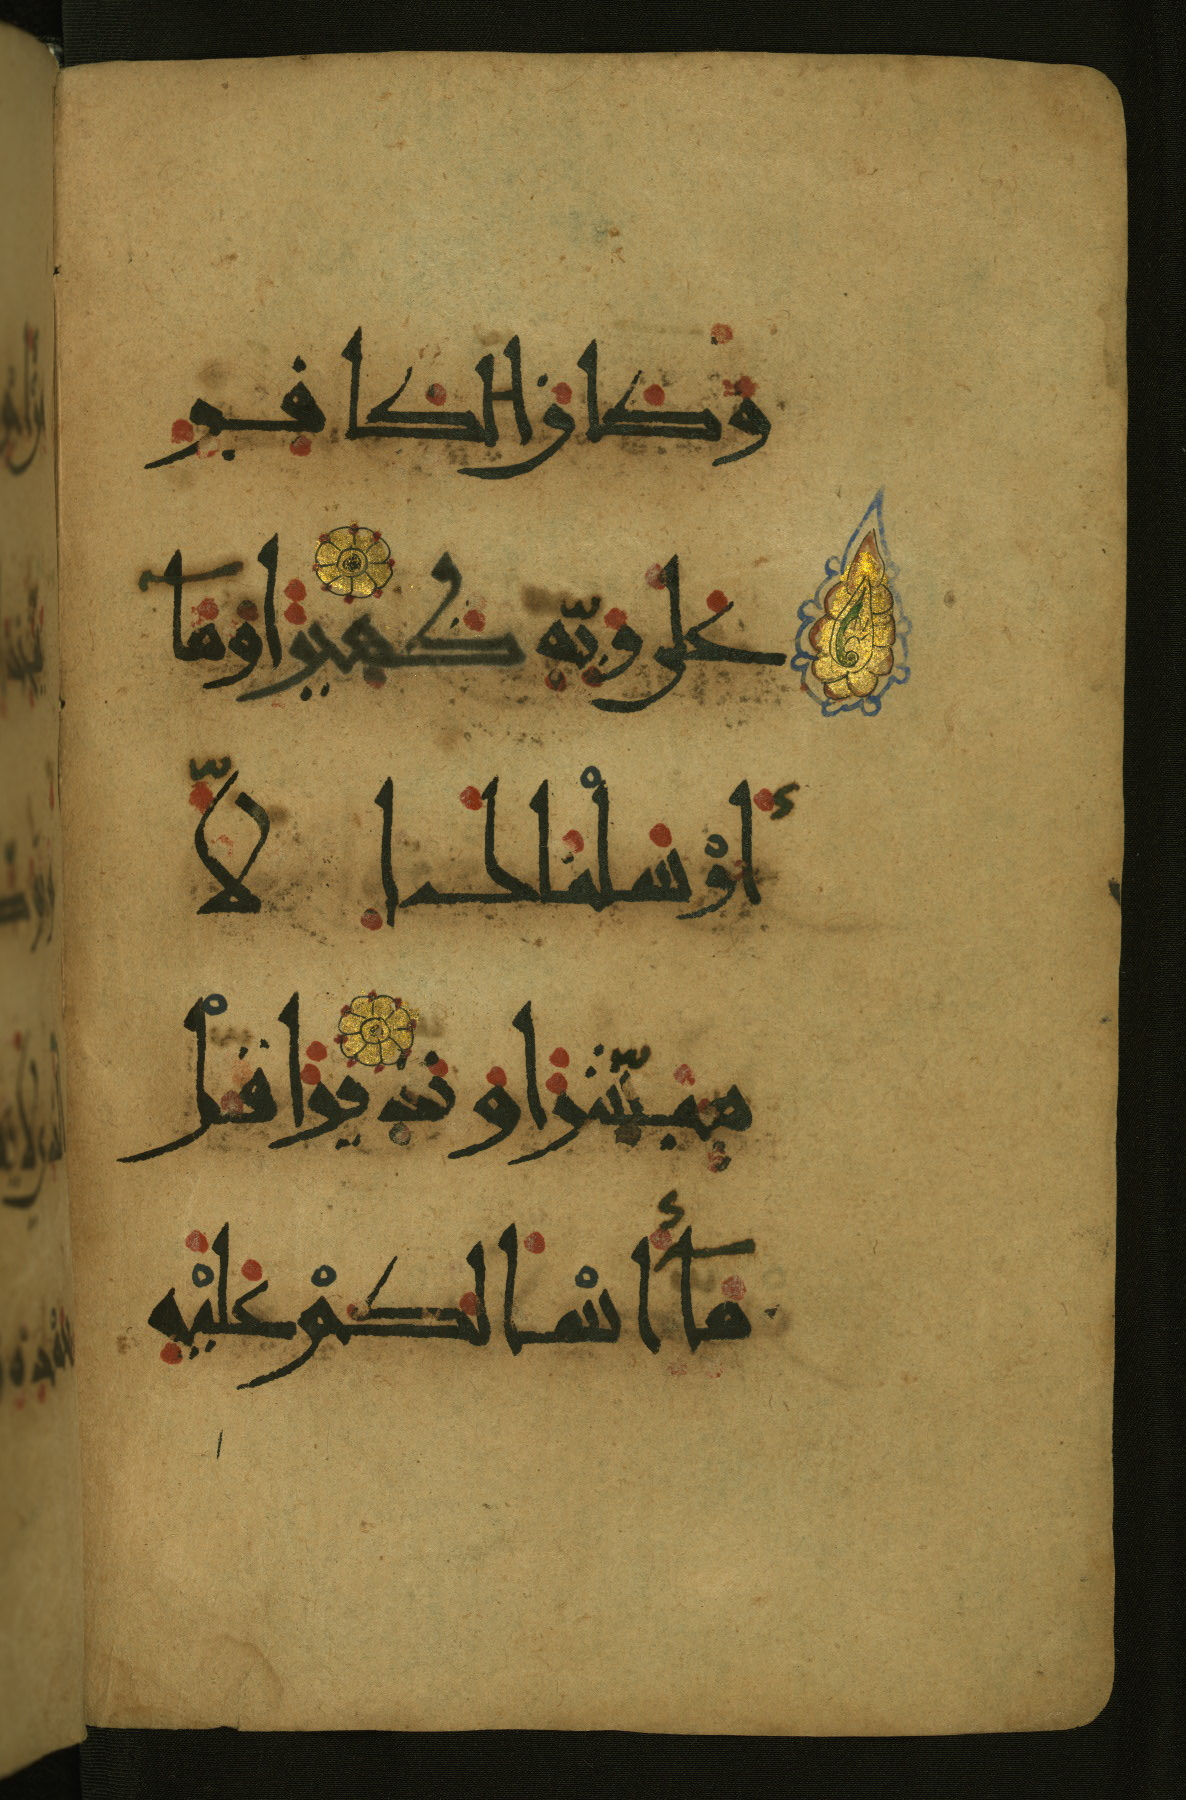
\includegraphics[height=0.4\textheight]{images/W555_000024_sap.jpg}
		\caption{Twelfth century CE \emph{qurʼān} in broken cursive or New Abbasid script (Walters W.555, fol. 10b)}
                \label{fig:ara_broken}
        \end{subfigure}
	\hfill
	\begin{subfigure}[t]{.55\columnwidth}
		\centering
                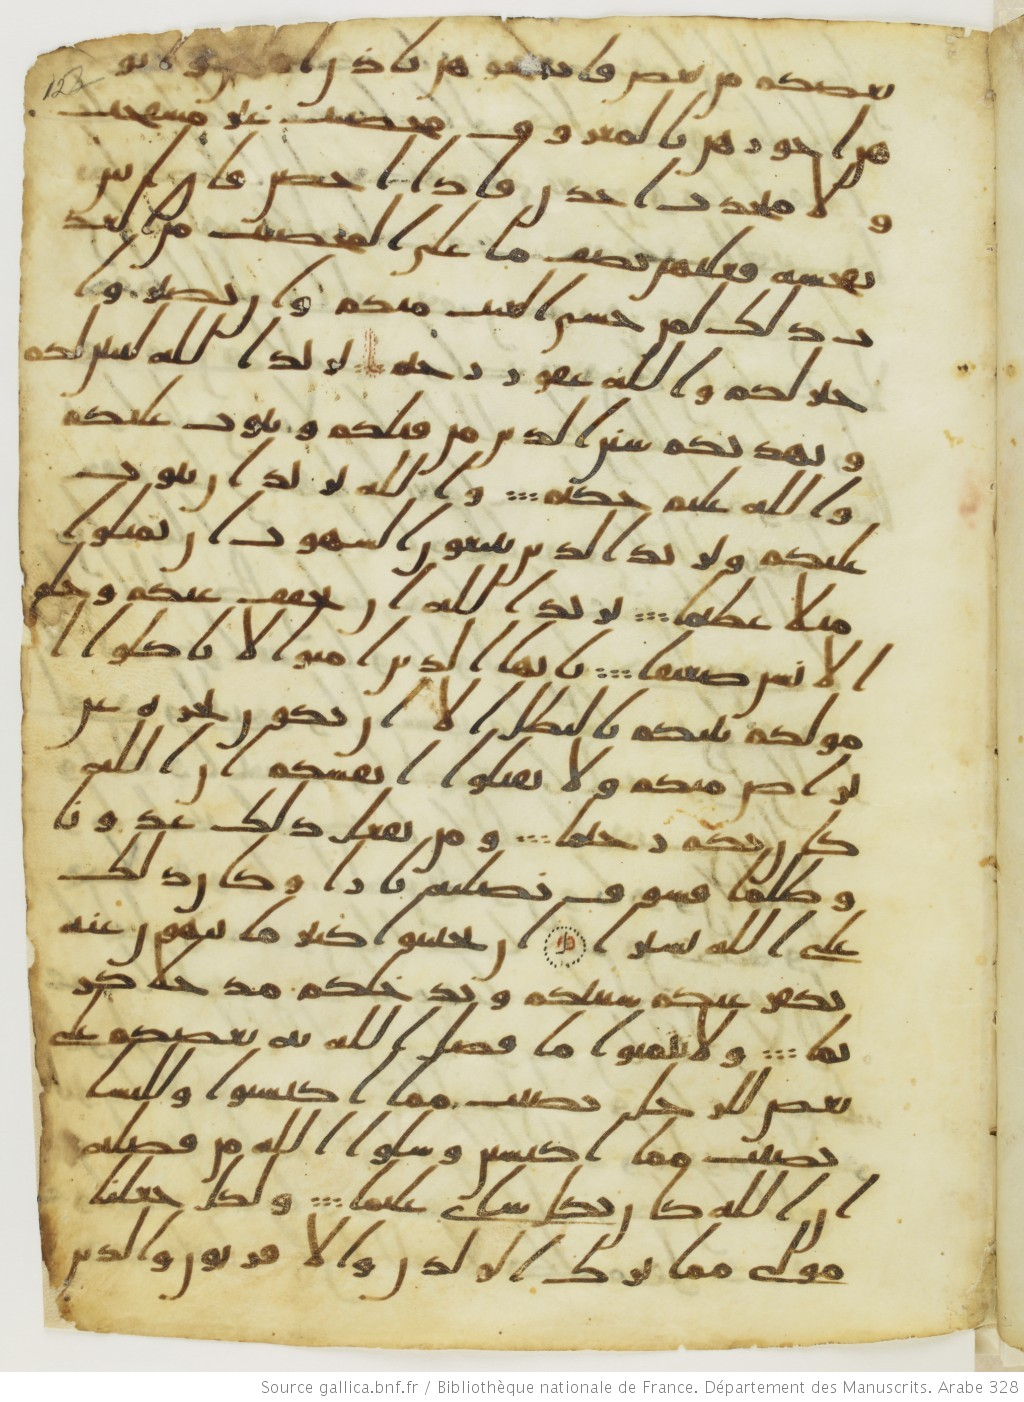
\includegraphics[height=0.4\textheight]{images/Coran__btv1b8415207g_31.jpeg}
		\caption{Seventh century CE \emph{qurʼān} in \emph{ḥijāzī} script (BnF Arabe 328, fol. 12r)}
                \label{fig:ara_hijazi}
        \end{subfigure}
        \caption{Early Arabic styles}
\end{figure}

By the tenth century CE the use of kufic in high status manuscripts began to be
replaced by a style known under a variety of names such as Eastern kufic, New
Abbasid Style, and broken cursive~\cite[pg. 144]{blair2006islamic}
(figure~\ref{fig:ara_broken}). This style was dominant into the thirteenth
century CE for copies of the \emph{qurʼān} when it was relegated to ornamental
purposes such as titles and headings. Similarly to older styles, it does not
represent a single hand but at least two different groups. The main
characteristics of this style is the marked difference between thick and thin
strokes~\cite[pg. 167-168]{gacek2009arabic}. From this period also dates the
practice of using long \emph{taṭwīl} elongation to mark the start of a new
section of text~\cite[pg. 165]{blair2006islamic}.

\subsection{The Six Pens}

The greatest impact on the evolution of Arabic calligraphy between the tenth
and thirteenth century is usually attributed to three great calligraphers: Ibn
Muqlah (d. 940 CE), Ibn al-Bawwab (d. 1022 CE), and Yaqut (d. 1298 CE). The
fundamental development of the period between the tenth and thirteenth century
is the system of proportioned scripts and the canonicalization of the various
rounded styles under this system. Ibn Muqla is attributed with developing the
first proportioned script, \emph{al-khatt al-mansūb}, that defined each
letter's dimensions in the unit of rhomboid dots, impressions left by the reed
pen on the writing surface, with \emph{alif} spanning a circle circumscribing
all other graphemes. While this system is most likely only a thirteenth century
CE attempt at reconstructing the hand of the famous calligrapher, as none of
his works survived, Ibn al-Bawwab is credited with canonicalizing the round
chancery scripts in use at the time using this system~\cite[pg. 158-160,
213]{blair2006islamic}. Finally, Yaqut popularized the six proportional styles
known as the \emph{Six Pens}, which later became the dominant scripts in the
East~\cite[pg. 251]{gacek2009arabic}.

These six styles are usually paired in three sets of one display (majuscule)
and one text (minuscule) script:

\begin{itemize}
	\item \emph{thuluth} with \emph{naskh}
	\item \emph{muḥaqqaq} with \emph{rayḥān}
	\item \emph{tawqīʿ} and \emph{riqāʿ}
\end{itemize}

\begin{figure}[h!tp]
        \centering
        \begin{subfigure}{\textwidth}
		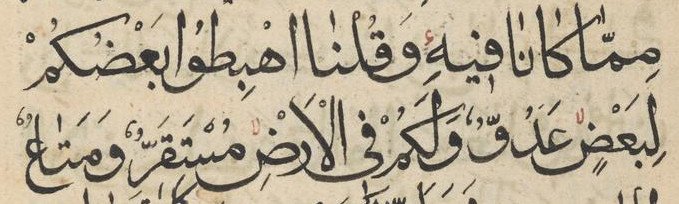
\includegraphics[width=\textwidth]{images/6940_0010_web.jpg}
		\caption{Two lines written in \emph{thuluth} from an undated copy of the \emph{qurʼān} (Columbia University, MS Or 234, fol. 4v).}
                \label{fig:ara_thuluth}
        \end{subfigure}
        \vskip\baselineskip
        \begin{subfigure}{\textwidth}
		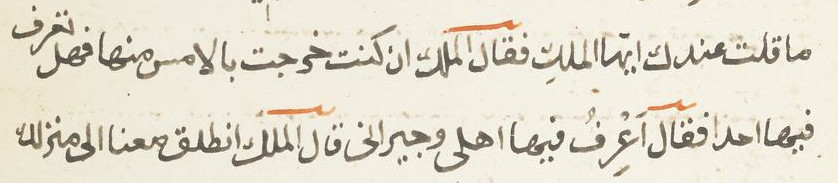
\includegraphics[width=\textwidth]{images/9224_0009_web.jpg}
		\caption{Two lines written in \emph{naskh} from an undated book of Qur’anic stories (Free Library of Philadelphia, Lewis O 170, fol. 5r).}
                \label{fig:ara_naskh}
        \end{subfigure}
        \vskip\baselineskip
        \begin{subfigure}{\textwidth}
		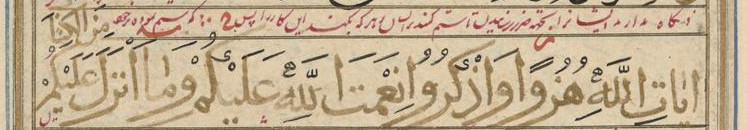
\includegraphics[width=\textwidth]{images/6937_0054_web.jpg}
		\caption{Central line in \emph{muḥaqqaq} in gold of a bilingual
		Arabic and Persian copy of the \emph{qurʼān}. The red line
		above is part of the interlinear Persian translation in
		\emph{nastaʼlīq} (Columbia University, Ms Or 222, 23r).}
                \label{fig:ara_muhaqqaq}
        \end{subfigure}
        \vskip\baselineskip
        \begin{subfigure}{\textwidth}
		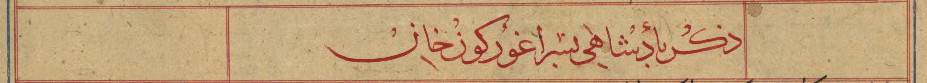
\includegraphics[width=\textwidth]{images/W676_000004_sap.jpg}
		\caption{Chapter heading written in  \emph{tawqīʿ} script from a fifteenth century CE Timurid history (Walters W.676, fol. Bb).}
                \label{fig:ara_tawqi}
        \end{subfigure}
        \vskip\baselineskip
        \begin{subfigure}{\textwidth}
		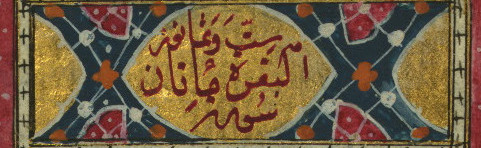
\includegraphics[width=\textwidth]{images/W567_000005_sap.jpg}
		\caption{Heading in \emph{riqāʿ} script of a nineteenth century CE \emph{qurʼān} copy (Walters W.567, fol. 2a).}
                \label{fig:ara_riqa}
        \end{subfigure}
	\caption{Samples of five of the Six Pens}
\end{figure}


\emph{Thuluth} (figure~\ref{fig:ara_thuluth}) is an ancient chancery script
although its exact features are unknown prior to its reform to the proportioned
script system in the eleventh century CE. Its most notable properties are
descenders which fall far below the baseline and curve upwards again for
certain letters, hairlines, and many contracted letterforms. As a display
script its letter are large but horizontally compact. In administrative use it
was utilized for important documents while in codices it was used mainly for
titles and chapter headings~\cite[pg. 275]{gacek2009arabic}.

\emph{Naskh} (figure~\ref{fig:ara_naskh})  is the most widely used book hand of
the Islamic East. It is a serifless script without unauthorized connections
between letters, long ascenders, and short descenders. Some Persian and Ottoman
variations of the script exist. It is the basis for most modern Arabic
typefaces intended for use in prose~\cite[pg. 162-163]{gacek2009arabic}.

\emph{Muḥaqqaq} (figure~\ref{fig:ara_muhaqqaq}) is one of the ancient scripts
originally devised before the proportioned scripts system. It is rectilinear,
i.e. only a small proportion of the penstrokes are curved or curvilinear. It is
a seriffed script with vocalization performed with a different pen, often in a
different color. While grouped as the display script to \emph{rayḥān} it also
became a bookhand for copies of the \emph{qurʼān} by the thirteenth century
CE~\cite[pg. 160-161]{gacek2009arabic}.

\emph{Rayḥān} is the smaller counterpart to \emph{muḥaqqaq}. The letter forms
were identical except for their size, the inclusion of serifs, and the
execution of vocalization with the same pen as the letters~\cite[pg.
308]{EncyclopediaofArabicLanguageandLinguisticsVolume3}.

\emph{Tawqīʿ} (figure~\ref{fig:ara_tawqi}) is a smaller diplay variant of the
\emph{thuluth} chancery script being written with even more hairlines. Like
\emph{thuluth} it was rarely used as a bookhand~\cite[pg.
264-264]{gacek2009arabic}.

\emph{Riqāʿ} (figure~\ref{fig:ara_riqa}) is the smaller version of the
\emph{tawqīʿ} script. It is optionally seriffed with slightly rightward
inclined \emph{alif}. In Iran the differences between it and \emph{tawqīʿ} were
minor with one publication using the terms synonymously~\cite[pg.
224]{gacek2009arabic}.

\subsection{Regional Styles}

Around the same period a number of regional scripts were developed. In the
Maghreb, Muslim Spain, and West Africa a number of scripts emerged that were
later summarized under the name \emph{maghribī}
(figure~\ref{fig:ara_maghribi}). These non-proportioned  hands are distinctive
but no detailled paeleographical analysis has been done to date and there exist
a number of sub-types. One shared feature is the use of a rounded nib resulting
in even thickness of strokes~\cite[pg. 147-148]{gacek2009arabic}.  The earliest
manuscripts in these styles date to the mid-tenth century CE with the earliest
surviving \emph{qurʼān} copy dated to 1008 CE but little change occured
afterwards~\cite[pg. 566]{blair2006islamic}.

Around the same time as Yaqut was refining the Six Pens, two new styles of
hanging scripts called \emph{taʿlīq} (figure~\ref{fig:ara_taliq}) and
\emph{nastaʼlīq} (figure~\ref{fig:ara_nastaliq}) emerged in Iran. These were
more suitable for writing languages such as Persian and Turkish that differ
from Arabic in their proportion of straight and curved letters. As such they
were never popular in the Arabic speaking world but \emph{nastaʼlīq} ended up
as the style of choice for a number of other states such as Ottoman Turkey and
Mughal India. The highly stylized \emph{taʿlīq} script with its curvilinear
elements, extraneous loops, and connected letter was a typical style for
official decrees, diplomatic correspondence, sometimes poetry, but almost never
codices, from the tenth century CE. The stereotypical \emph{taʿlīq} document
contains widely spaced lines with dramatic upward curving at the end of the
line. A variant broken \emph{taʿlīq} replaced it from the fourteenth century CE
in administrative use~\cite[pg. 270-273]{blair2006islamic}.

\begin{figure}[h!tp]
        \centering
	\begin{subfigure}[t]{.48\columnwidth}
		\centering
                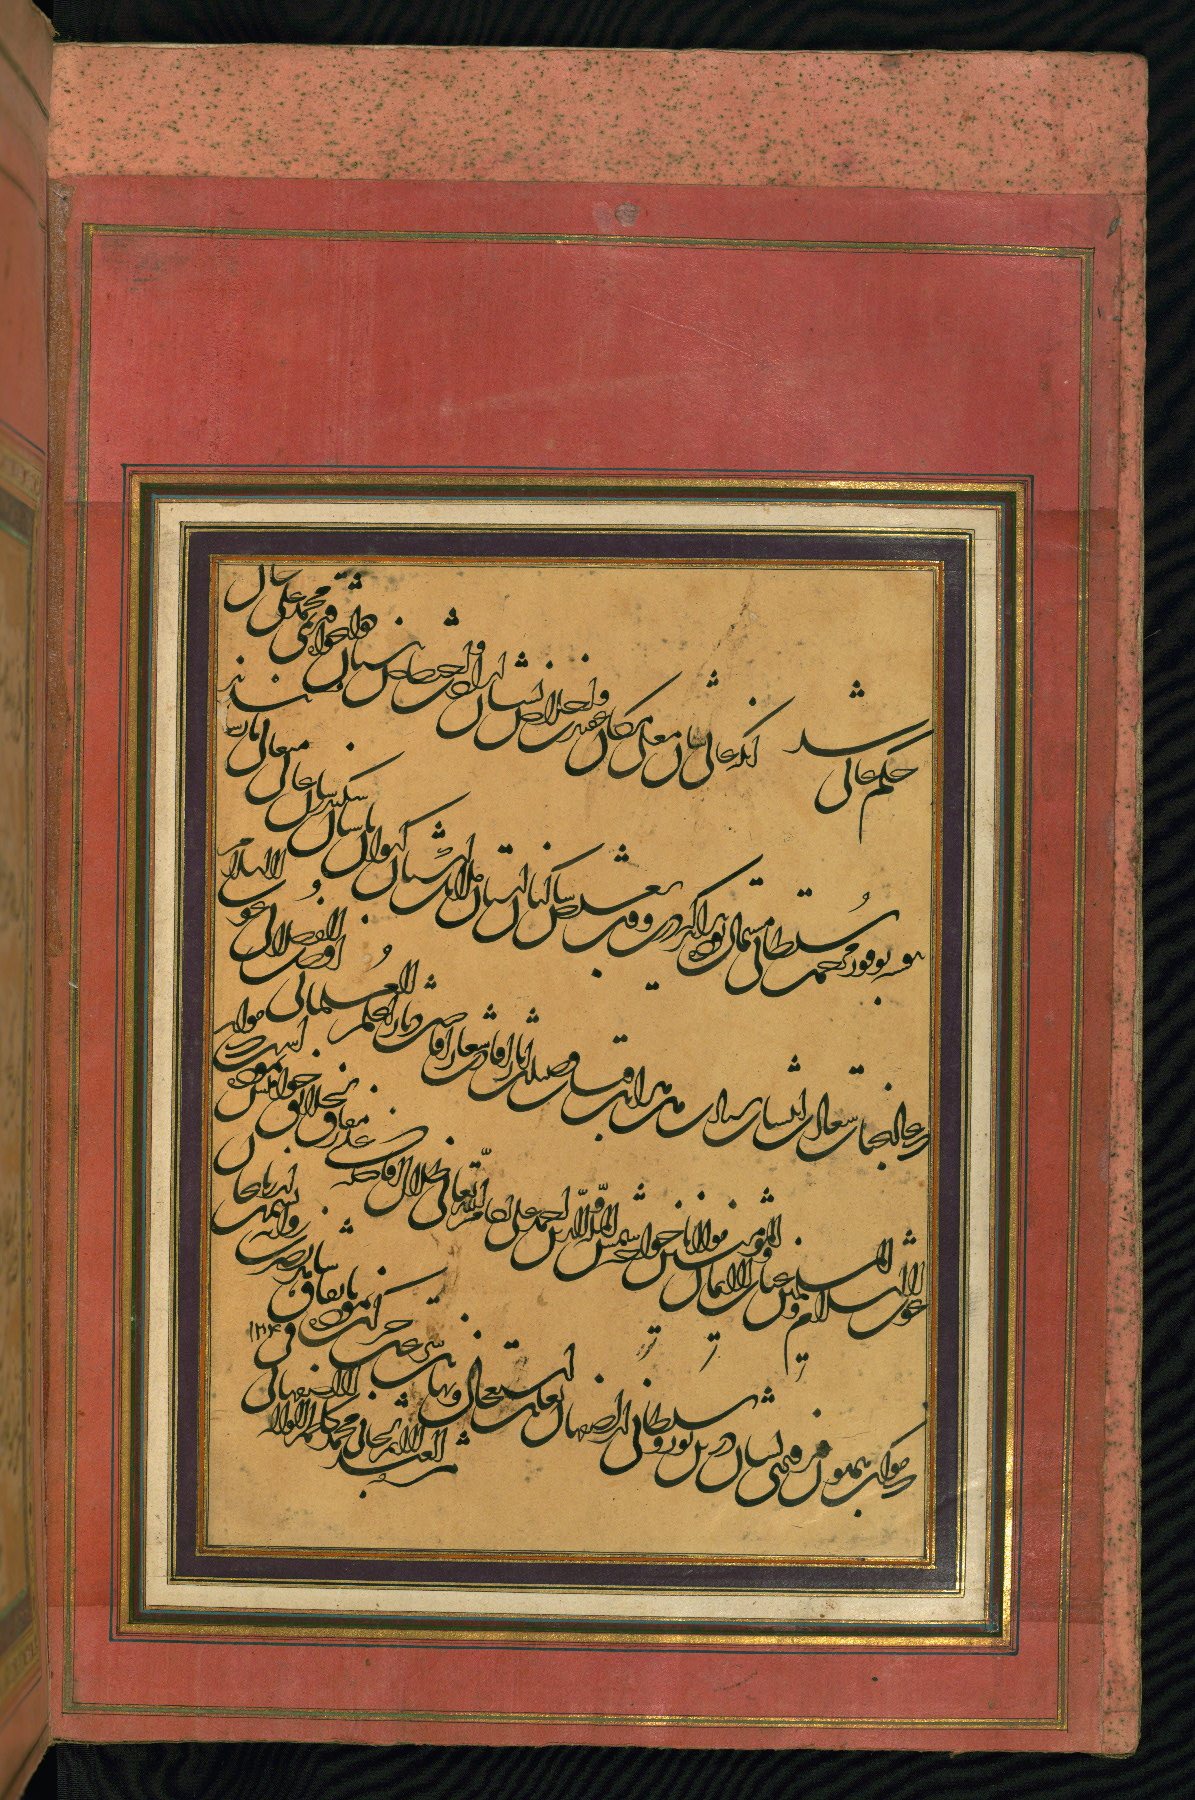
\includegraphics[height=0.43\textheight]{images/W670_000040_sap.jpg}
		\caption{Page from a Persian nineteenth century CE album of calligraphic samples written in \emph{taʼlīq} (Walters W.670, fol. 19b)}
                \label{fig:ara_taliq}
        \end{subfigure}
	\hfill
	\begin{subfigure}[t]{.48\columnwidth}
		\centering
                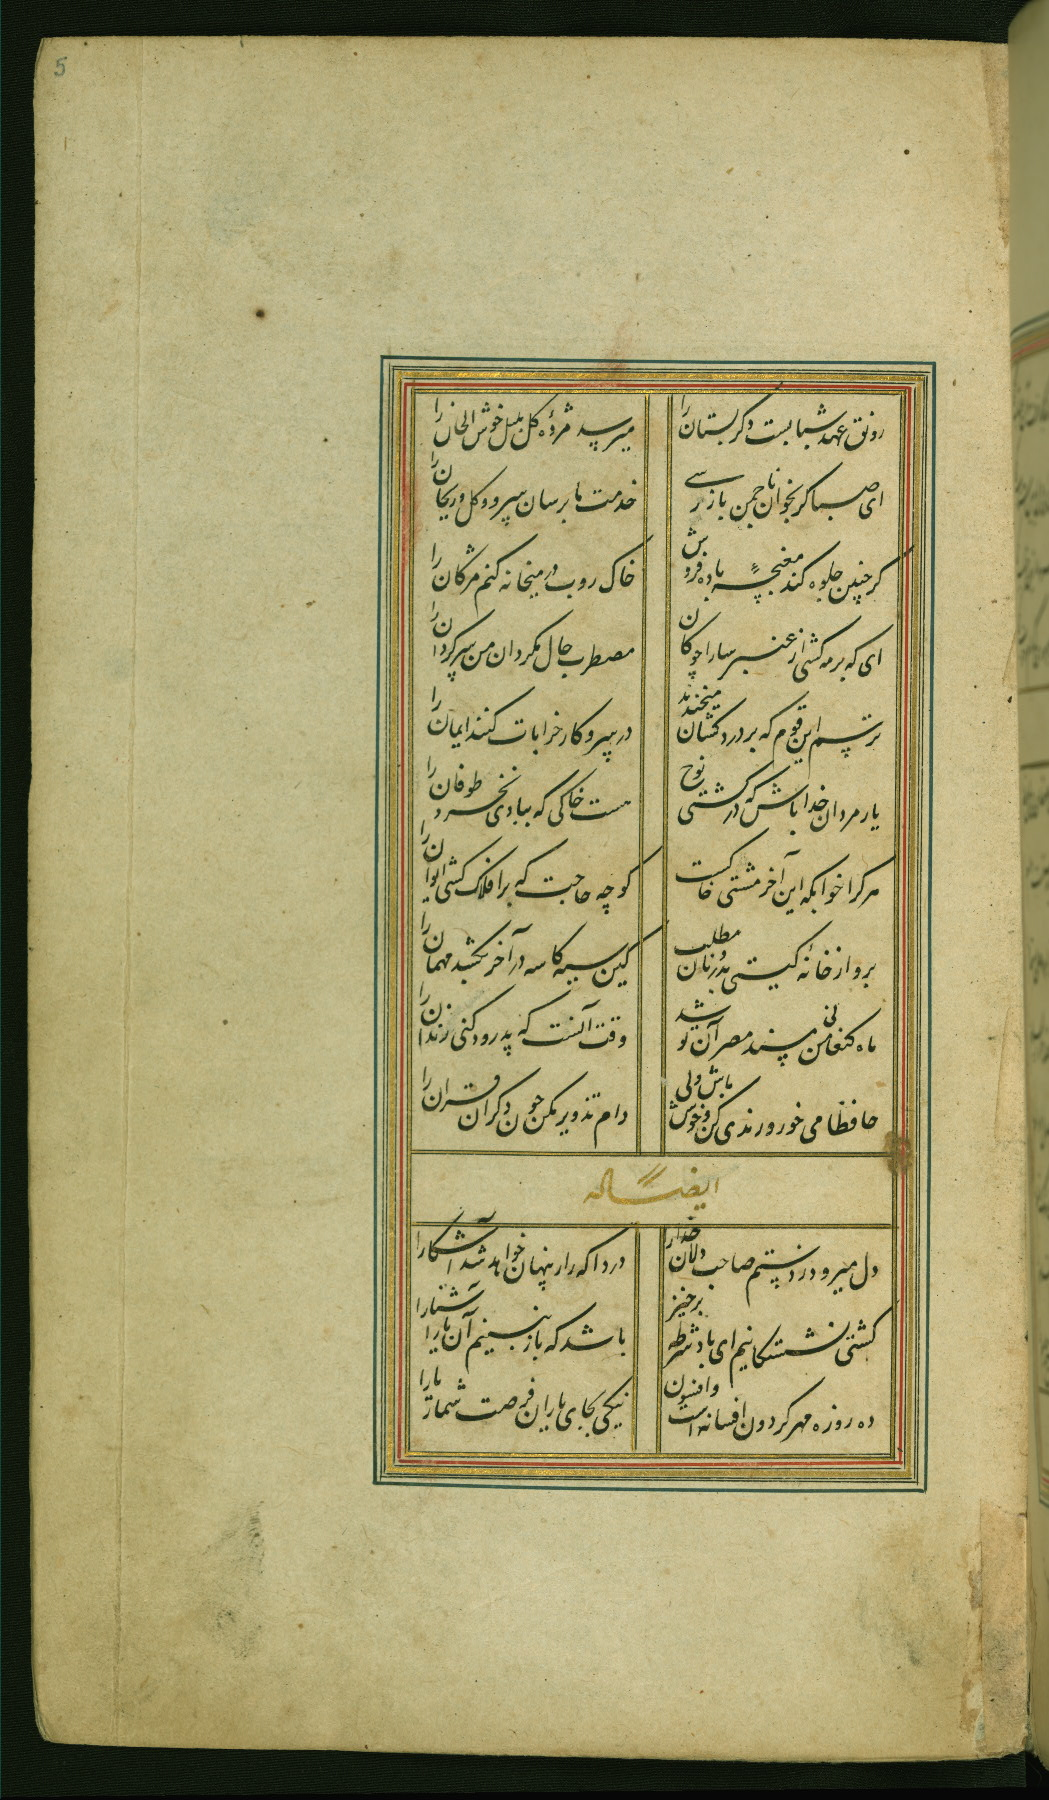
\includegraphics[height=0.43\textheight]{images/W631_000014_sap.jpg}
		\caption{1539 CE page from a collection of poems written in \emph{nastaʼlīq} (Walters W.631, fol. 5a)}
                \label{fig:ara_nastaliq}
        \end{subfigure}
        \vskip\baselineskip
	\begin{subfigure}[t]{.48\textwidth}
		\centering
		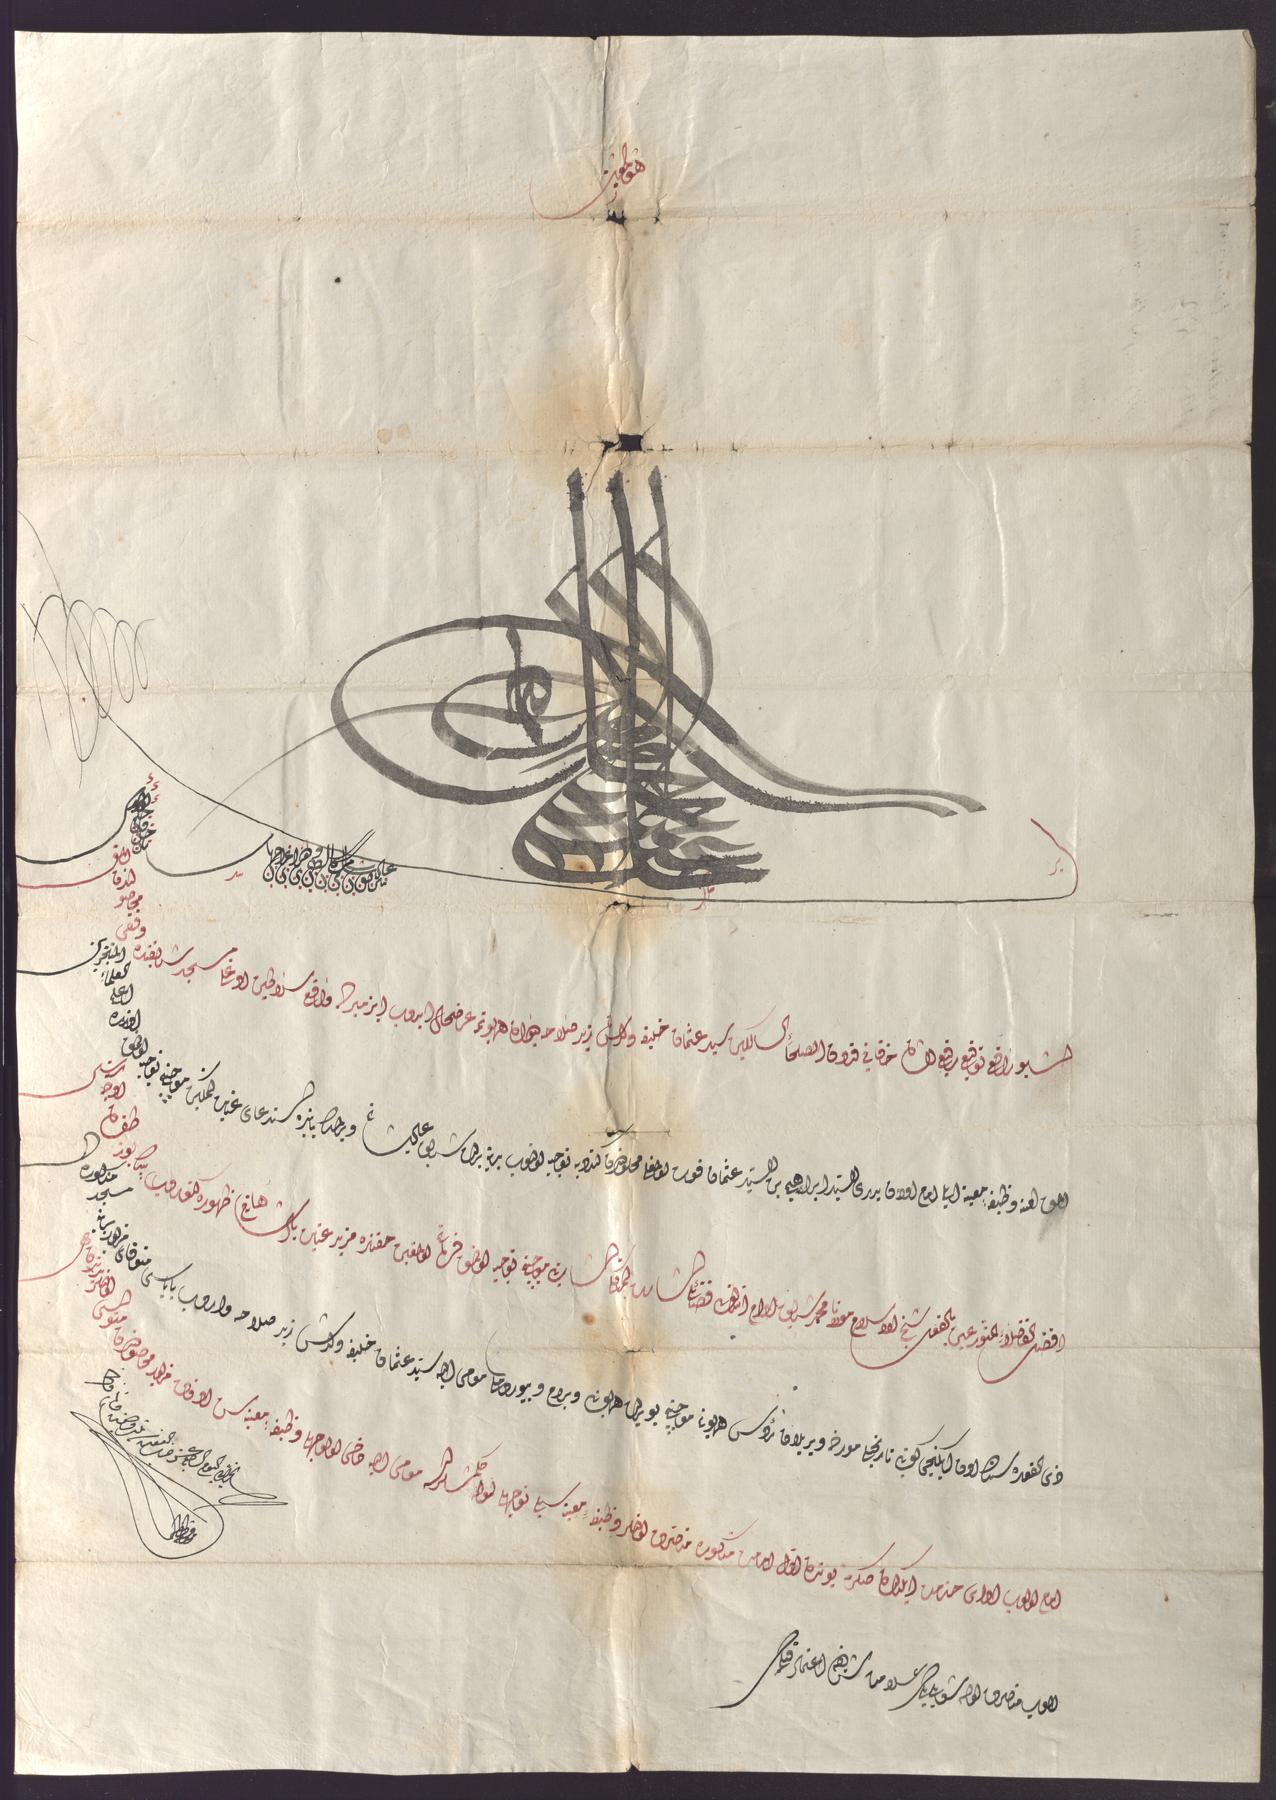
\includegraphics[height=0.4\textheight]{images/9676_0002_web.jpg}
		\caption{1779 CE Ottoman firman \emph{diwānī} script (American Philosophical Society Ms. Coll. 200, fol. 2)}
                \label{fig:ara_diwani}
        \end{subfigure}
	\hfill
	\begin{subfigure}[t]{.48\textwidth}
		\centering
                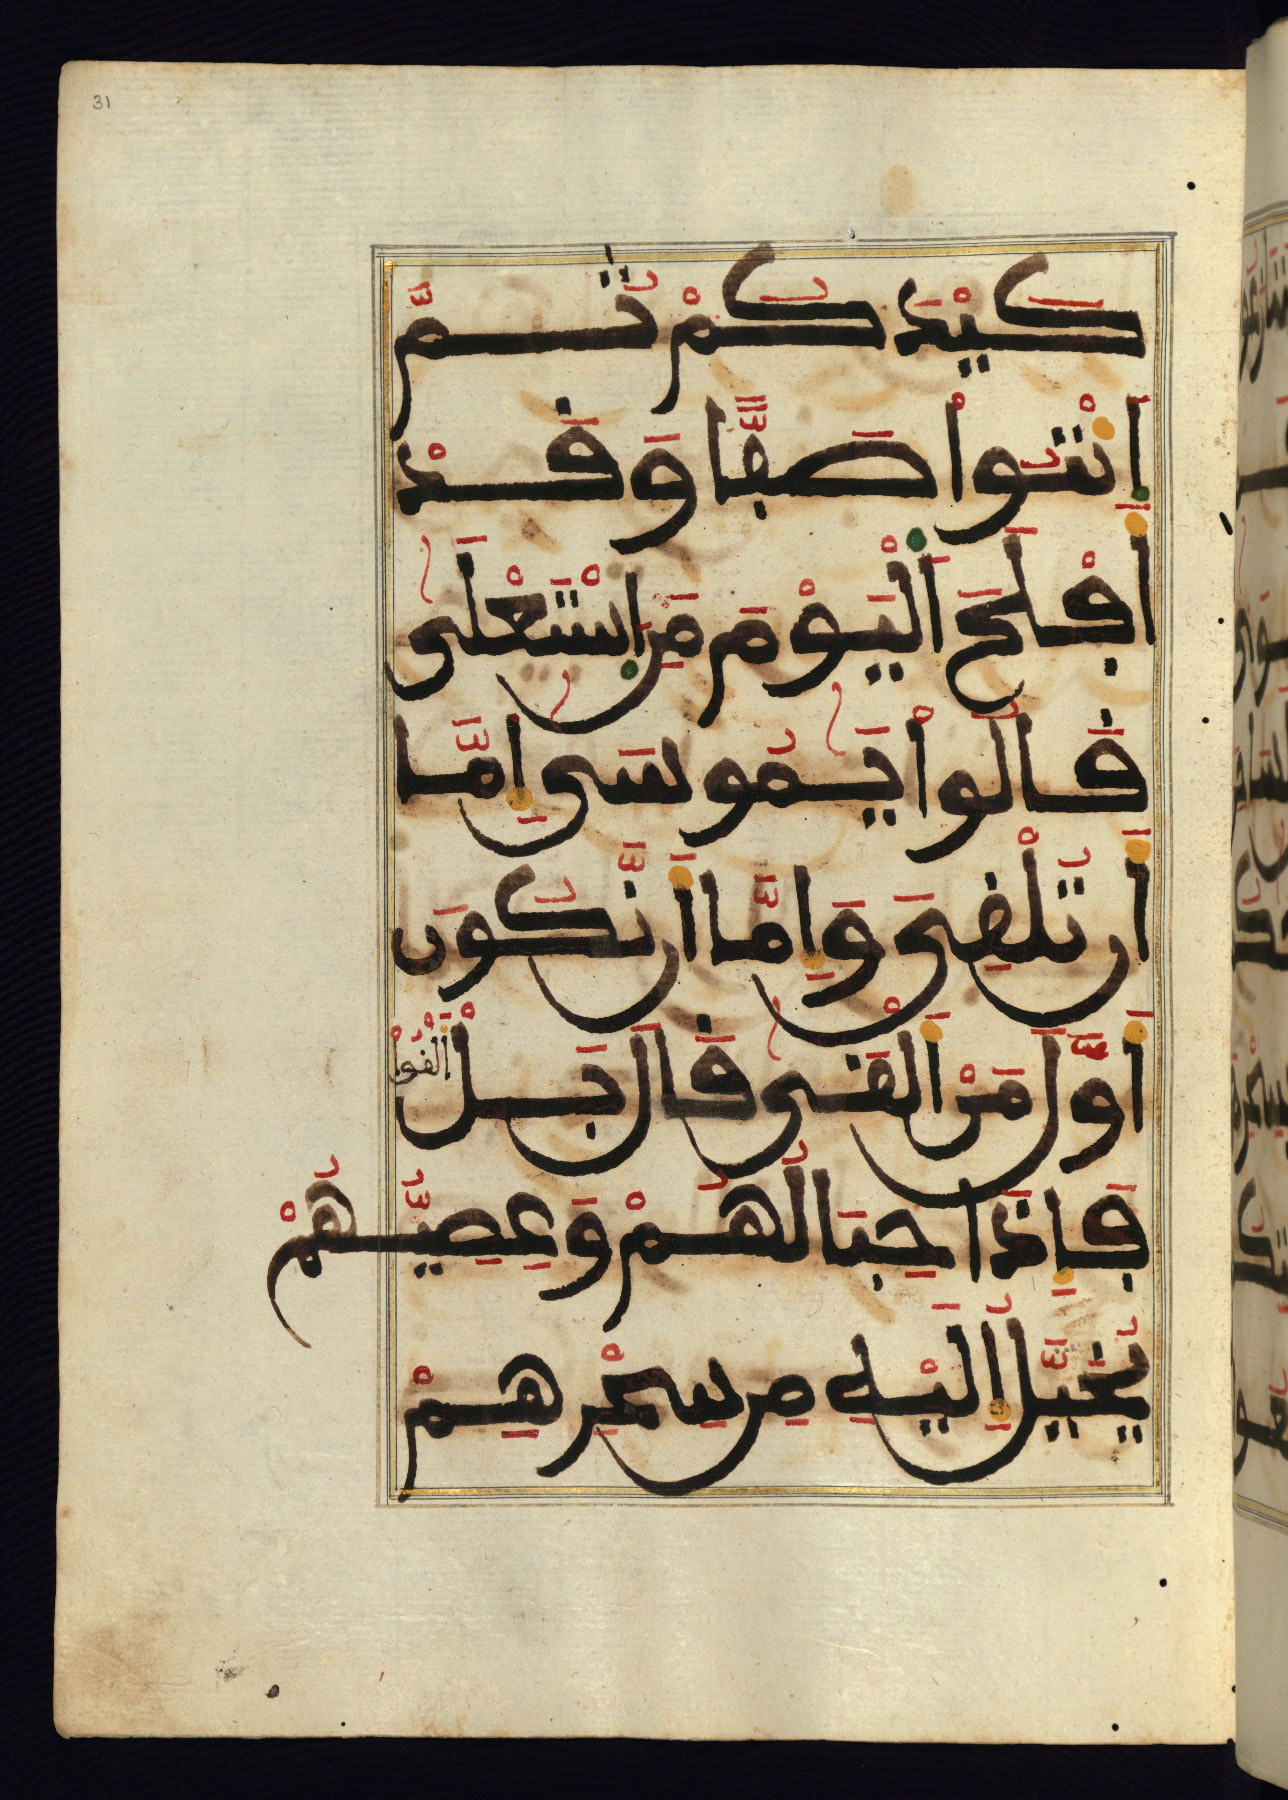
\includegraphics[height=0.4\textheight]{images/W568_000064_sap.jpg}
		\caption{Nineteenth century CE \emph{qurʼān} in large \emph{maghribī} script (Walters W.568, fol. 31a)}
                \label{fig:ara_maghribi}
        \end{subfigure}
        \caption{Example of regional styles}
\end{figure}


The second major Persian style, \emph{nastaʼlīq}, became the epitome of Persian
literature. At first reserved for poetry, it took over the place of
\emph{naskh} for prose by the fifteenth century as well. It is characterized by
individual words descending onto a common baseline, greatly elongated
horizontal lines, and the aforementioned heaping of the last stroke~\cite[pg.
166-167]{gacek2009arabic}. While the aforementioned styles, depending on the
preservation of the document, the desired generalization, and accuracy, are not
inherently troublesome for a modern OCR engine, the sophistication displayed by
the most decorated \emph{nastaʼlīq} epics and calligraphic specimens are highly
challenging. Calligraphers of the time were interested in variety and visual
excitement, arranging verses on the diagonal, changing direction between
successive verses, alternating red, blue, orange, and green inks for headings,
and adding lavish illumination and scrollwork. The writing was being subsumed
by decoration~\cite[pg. 436]{blair2006islamic}. 

Round scripts, primarily \emph{naskh} and \emph{thuluth}, and Persian hanging
scripts were common in the Ottoman Empire with their relative proportion in
text production varying over the centuries\footnote{\cite[chapter
XI]{blair2006islamic} elaborates the cycles of popularity between round and
hanging scripts.} In the fifteenth century CE imperial scribes began to develop
the \emph{taʿlīq} script into the highly stylized \emph{diwānī}
(figure~\ref{fig:ara_diwani}) chancery style with its unauthorized connections
between letters and curved baselines.

\section{Printing}

Notwithstanding the fact that this dissertation is mostly concerned with
handwritten text recognition, printing deserves some consideration. This is
especially true given that the development and diffusion of printing is
directly linked to the practice of calligraphy. Printing is the mechanical
reproduction of text and images. Since Johannes Gutenberg developed his
printing system around 1450 CE, the term has been mostly referring to movable
type printing, where reverse images of different graphemes (including
punctuation marks and decorations) are cast in metal as individual elements
(types). Types are arranged into larger units (most often entire lines), which
are then assembled into a matrix to create a full page. The matrix thus created
is then placed in a printing press. It is inked and brought into contact with
the material to be printed, usually paper. The process can be repeated as many
times as desired. Nevertheless, it should be noted that other kinds of
printing, such as Egyptian and Mesopotamian cylinder seals as well as Chinese
woodblock printing, have pre-existed Gutenberg's invention by thousands of
years. 

Unlike movable type printing, block printing employs a unitary matrix which is
carved out of a single piece of wood. The production of block-printed texts is
attested throughout the Islamic world since at least 900 CE, although the
practice seems to have died out by 1430 CE. The extent to which this technique
was actually used and where it exactly originated from is still unknown. Few
block-printed documents can be found in existing archives, and there is a lack
of archeological evidence related to matrices and printing equipment, which
leaves the topic shrouded in obscurity. Amulets and charms are the only
documents that have been regularly preserved. They contain Quranic passages
printed on paper in a wide array of styles, and generally follow similar
calligraphic practices as their handwritten counterparts \footnote{A survey of
the current state of scholarship is found in \cite{schaefer2006enigmatic}}.
They have not attracted much academic interest, and the DIA community has not
developed any specific methods to treat them. 

Movable type printing reached the Islamic world at the end of the fifteenth
century CE with the establishment of printing presses in Constantinople and
other cities of the Ottoman Empire. However, they were run by and for the
Jewish minority and did not produce books in Arabic script. It is often assumed
that the Ottoman Sultan Bayezid II prohibited movable type printing outright,
or restricted it to certain scripts or minorities living in the Empire in 1485
CE. However, evidence is slim and contradictory \cite{schwartz2017did}. What is
certain is that printing of the Arabic script in the Islamic world was first
performed in 1727 CE, in a workshop established by imperial printer Ibrahim
Müteferrika. It does not mean that Arabic books were not printed, as imports
did exist, mostly from Italian workshops. The earliest example of this is a
1513 CE book of hours printed in Venice by Gregorio de
Gregori~\cite{krek1979enigma}. The \emph{qurʼān}'s earliest printed edition was
produced in 1537-1538 CE by two brothers, Paganino and Alessandro Paganini. It
proved to be an utter commercial failure because of its odd typeface and of the
numerous errors the text contained \cite[pg. 219-220]{bloompaper}. Later,
famous type-founders such as Robert Granjon (1585 CE), William Caslon (1720
CE), or Giambattista Bodoni (1759 CE) made other attempts at cutting typefaces.
However, even these proved to be simplistic and of low
quality~\cite{tracy1975advances}. 

Although universally derided for their lack of grace, legibility, and
orthographical correctness later imports seem to have found more popular
acceptance as lamented by Muteferrika in a 1727 CE work on the usefulness of
printing. The secular nature of the vast majority of these imports support the
theory that religious sentiment was a principal factor hindering the adoption
of printing, although the economic interests of a substantial class of scribes
and calligraphers certainly played a role, in addition to the inherent
difficulties of creating adequate typefaces for a cursive script~\cite[pg.
605]{blair2006islamic}.

Despite this multi-faceted resistance to movable type printing, some refinement
took place. While typeface cut in the Christian world were largely modelled on
the \emph{maghribī} style, Muteferrika introduced the more legible \emph{naskh}
style in printing which remains to this day the most popular style for printed
Arabic texts. However, creating a full Arabic font remained a truly staggering
task; the Imprimerie Nationale's twenty-four-point nineteenth century CE Arabic
typeface contained 710 different types~\cite[pg. 218]{bloompaper}. In addition,
actually setting such large typefaces required skill incomparable to the much
simpler Latin script. It has been argued that apart from social objections, the
sheer laboriousness combined with a lacking industrial base made movable type
printing uneconomical in the Islamic world \cite{auji2017neither}. Indeed, the
rise of printing presses in the nineteenth century coincides with the invention
of lithography which allowed inexpensive, accurate reproductions of handwritten
texts, missionary activity and modernization drives less subject to immediate
economic pressures \cite{turner1996dictionary}. Printers like Fāris al-Shidyāq,
founder of the al-Jawā’ib press in Istanbul, introduced Western-style layouts
with punctuation marks and paragraphs but were not able to resolve the
laborious typesetting process or aesthetic issues such as lacking overlap of
letters, line justification limited to baseline stroke elongation instead of
the more aesthetically pleasing letter elongation or stacking, and visible gaps
between individual types~\cite[pg. 605]{blair2006islamic}. The invention of hot
type line casting machines such as the 1911 Arabic Linotype eliminated gaps
between glyphs but the limits of the machine did not allow proper placement of
vowel marks~\cite[pg. 67]{nemeth2017arabic} and subsequent iterations
economised more and more glyph variants reducing the visual appeal of the final
product. Only the advent of software-driven phototypesetters in the 1960s make
sufficiently large type repertoires including contextual and elongated forms
economically feasible. Even though the last vestiges of the limitations of
physical type have disappeared with purely digital typesetters, most common
typefacess do not make use of these.

In the next chaper, we take a closer look at the limitations of current OCR
technology on modern printed Arabic texts.

\section{Basic requirements for Arabic OCR systems}

To summarize, the recognition of Arabic handwritten texts requires a number of
design decisions and features that available OCR engines do not have. This
dissertation could not address all of the required decisions and features,
chiefly because of the lack of available Arabic-script or substitute training
data. The main necessary features are presented below, by order of processing
inside a typical pipeline: 

\begin{description}
	\item[Freedom of Binarization] A number of reasons makes it impossible
		to devise a general binarization method that could apply to
		most Arabic handwriting: the variety of supports used to write
		Arabic, the often fragmentary nature of writing on papyrus, the
		presence of faded and acid-damaged writing in iron-gall inks,
		and the highly decorated nature of pages. While trainable
		methods using semantic segmentation approaches exist,
		oftentimes their training data requirements are insurmountable.
	\item[Segmentation of curved and slanted lines] The frequent use of
		baseline curvature and slanted lines for both practical and
		aesthetic purposes requires a layout analysis (LA) method
		capable of modelling lines in a way that allows normalization
		of the axis of writing and the effective suppression of
		non-line content.
	\item[Semantic layout analysis] Many Arabic manuscripts contain an
		unusual amount of paratext or textual \emph{noise}, be it
		marginal notes, parallel texts, interlinear translations, or
		detached word fragments. Proper treatment of these elements,
		e.g. separation of commentary from maint text or selection of
		the appropriate recognition model for a parallel text in
		another script, requires at least in part awareness of these
		elements in the LA component. As the types of elements, their
		presentation, and frequency can vary immensely it is highly
		desirable for the LA system to be trainable.
	\item[Advanced reading order determination] Related to the
		classification of textual components in the LA module is the
		correct ordering of the texts and the proper linking of
		paratextual components to the main text. As mentioned before
		this is a nacent field of research and all OCR systems
		available infer the order of text using highly flawed
		heuristics.
	\item[Segmentation-free transcription] The cursive nature of Arabic
		writing, particularly the variation of letter connections
		encountered between different scripts makes reliable
		segmentation into single graphemes impractical for handwritten
		texts, especially so when executed in highly stylized and
		contracted scripts. While a significant body of literature has
		focused on this problem, the success of sequence-to-sequence
		machine learning models that require no or only implicit
		segmentation/alignment of input image data and characters has
		by and large solved it.
	\item[Data creation and curation tools] While they are not directly
		part of OCR pipe\-lines (especially if employed in large-scale
		archival or library digitization projects), the lack of adapted
		open tools to create training data that can capture the
		pertinent features of Arabic handwritten text; and the
		subsequent lack of training data sets available for DIA
		research have stifled the field. Simple transcription tools
		such as those used in the studies detailed in
		chapter~\ref{ch:champs} are inadequate for preparing
		multi-purpose datasets. Fully featured Virtual Research
		Environments (VREs) for palaeographic scholarly work are one
		way of reaching deeply annotated data through flexible
		non-writing-system-specific data models.
\end{description}

Other minor technical requirements which are not large enough to be the focus
of a dedicated research question are sometimes disregarded. The most visible
example of this is the lack of support, in older or purely research software,
for non-ASCII and bidirectional text requiring manual substitution and
reordering of code points. More subtle sources of errors such as overly
aggressive normalization of input text, lack of Unicode whitespace
normalization, and the treatment of non-printing code points are also prevalent
and often difficult to ascertain, especially in proprietary software. 

It should be noted that while the underlying motivations to implement the above
requirements are specific to the Arabic script, comparable situations exist for
documents written in other scripts. De facto, similar motivations for
bin\-ariz\-a\-tion-freedom apply to almost any historical written document; not to
mention curved handwriting, marginalia, and parallel texts. Therefore, research
which focuses on tailoring an OCR system capable of better processing Arabic
texts is also likely to \emph{enhance} the capacity to process other texts as
well.

\phantomsection
\printbibliography[heading=subbibliography]
\endrefsection
